% !TeX program = xelatex
% =====================================================================
% ROZPRAWA DOKTORSKA (język polski; publikacje po angielsku)
% „Warunki przyczynowości i wycieki danych w strumieniowej ewaluacji
%  detektorów na grafach komunikacji"
%
% Rozdziały:
%   1. Wstęp
%   2. Przegląd literatury
%   3. Rozdział formalny (na bazie formal_chapter.tex)
%   4. Lateral phishing jako naruszenie grafu komunikacji (art. A, JNCA)
%   5. Spear phishing jako naruszenie grafu wiedzy domenowej (art. B, IEEE)
%   6. Synteza
%   7. Zakończenie
%
% Kompilacja: tectonic main.tex  (XeTeX + polyglossia + natbib/bibtex)
% =====================================================================
\documentclass[12pt,a4paper,oneside]{report}

\usepackage{amsmath,amssymb,amsthm}
\usepackage{booktabs}
\usepackage{multirow}
\usepackage{graphicx}
\usepackage{polyglossia}
\setmainlanguage{polish}
\usepackage{fontspec}
\usepackage[numbers,sort&compress]{natbib}
\usepackage[colorlinks]{hyperref}

\graphicspath{{figures/}}

% ---- obiekty formalne (nagłówki zgodne z rozdziałem 3) --------------
\newtheorem{theorem}{Twierdzenie}[chapter]
\newtheorem{proposition}[theorem]{Stwierdzenie}
\newtheorem{lemma}[theorem]{Lemat}
\newtheorem{corollary}[theorem]{Wniosek}
\newtheorem{definition}[theorem]{Definicja}
\newtheorem{remark}[theorem]{Uwaga}
\newtheorem{example}[theorem]{Przykład}

% ---- makra (jak w formal_chapter.tex) -------------------------------
\newcommand{\E}{\mathbb{E}}
\newcommand{\Prob}{\mathbb{P}}
\newcommand{\R}{\mathbb{R}}
\newcommand{\event}{\mathbf{e}}
\newcommand{\strict}{\prec}

\title{Warunki przyczynowości i wycieki danych\\
w strumieniowej ewaluacji detektorów na grafach komunikacji}
\author{Kamil Warpechowski}
\date{listopad 2026}

\begin{document}

\maketitle

\begin{abstract}
Rozprawa traktuje phishing ukierunkowany (lateral phishing z przejętego konta
oraz impersonację zewnętrzną typu BEC) jako naruszenie grafów organizacji:
grafu komunikacji i grafu wiedzy domenowej. Teza rozprawy jest dwojaka.
Po pierwsze, sygnał detekcyjny dla ogona ukierunkowanego mieszka w dynamice
czasowej i strukturalnej tych grafów, nie w treści pojedynczej wiadomości:
odbiorcza fala kaskady (temporal GNN, AUC 0.90; degradacja łagodniejsza niż
detekcji wolumetrycznej pod atakiem skrytym) oraz niespójność międzywarstwowa
multipleksu (AUC 0.70$\to$0.87, likwidacja fałszywych alarmów na legalnych
nowych nadawcach). Po drugie, empiryczny wynik detektora strumieniowego mówi
cokolwiek o warunkach produkcyjnych tylko pod czterema warunkami
przyczynowości: przyczynowości zdarzeniowej cech, rozłączności podziału po
ofiarach, usunięciu brzegowej sygnatury czasu i realistycznej fabrykacji
śladów; naruszenie każdego z nich powoduje zawyżenie raportowanych liczb, co rozprawa
pokazuje formalnie (twierdzenia i konstrukcyjne kontrprzykłady) i empirycznie
(pułapka wycieku rytmu: pozorna czułość 0.73 spada do 0.00 pod uczciwym
podziałem czasowym). Wszystkie liczby pochodzą z paczki reprodukcyjnej
(code/results/*.csv); wyniki walidowano na realnych grafach komunikacji
(Enron, email-Eu-core, CollegeMsg).
\end{abstract}

\tableofcontents

% =====================================================================
% ROZDZIAŁ 1 — Wstęp
% =====================================================================
\chapter{Wstęp}
\label{rozd:wstep}

\section{Problem i motywacja}
\label{sec:w-problem}

W poniedziałek rano przejmowane jest konto pocztowe pracownika. Zanim
doba się skończy, jego kontakty w dwóch działach i w firmie partnerskiej
otrzymują krótką, wiarygodną wiadomość z linkiem --- każda od kolegi, z
którym korespondują co tydzień; część z nich klika, a godzinę później
ich własne kontakty otrzymują tę samą wiadomość. Żaden pojedynczy
element żadnej z tych wiadomości nie zdradza oszustwa
\citep{butavicius2022why,sturman2025security}. To \emph{lateral phishing}:
kampania wysłana z prawdziwego, wewnętrznego konta przejętego przez
atakującego; w skali systemowej scharakteryzowali go \citet{ho2019detecting}
jako ataki docierające do wielu odbiorców wewnątrz i wokół organizacji.
Raporty FBI IC3 szacują straty spowodowane przez Business Email Compromise
(BEC), którego lateral phishing jest odmianą „od środka", na około
2{,}9 miliarda dolarów w~2023 roku \citep{fbi2024ic3}.

W drugim scenariuszu, lustrzanym wobec pierwszego, na skrzynkę dyrektora
finansowego trafia prośba o pilny przelew od „prezesa". Treść jest
dopracowana, pretekst wiarygodny, a nadawca --- zewnętrzny --- respektuje
wszystko, czego adresat oczekuje: właściwe nazwisko, właściwy projekt,
właściwy ton \citep{dewan2014analyzing,brown2025web}; koszt takiej
personalizacji językowe modele obniżają z każdym rokiem
\citep{bethany2024evaluating}. To \emph{impersonacja zewnętrzna}, czyli
spear phishing w reżimie BEC.

Detekcja phishingu bywa przedstawiana jako problem niemal rozwiązany.
Nowoczesne filtry, oparte na treści i reputacji, klasyfikują kampanie
masowe z dokładnością $\sim$98\% na typowych benchmarkach
\citep{birthriya2025detection,tan2020graph}. Liczba ta jest jednak
myląca: dokładność na benchmarkach jest zdominowana przez ogon masowy,
podczas gdy rzadki ogon ukierunkowany --- spear phishing i BEC ---
napędza większość strat finansowych \citep{cidon2019high,ho2019detecting},
jednocześnie z definicji omijając metody oparte na treści. Lateral phishing
jest najtrudniejszym przypadkiem tego ogona: przejęte konto przechodzi
każdą kontrolę tożsamości, reputacji czy relacji, bo wszystkie one są
prawdziwe. W obu scenariuszach oszustwo nie leży w tym, \emph{co} jest
napisane, lecz w tym, \emph{kto} pisze \emph{kiedy} --- i co dzieje się
potem.

\section{Teza rozprawy}
\label{sec:w-teza}

Rozprawa broni następującej tezy, sformułowanej w dwóch częściach.

\begin{description}
\item[T1 (sygnał).] Phishing ukierunkowany --- zarówno w wariancie lateral
(przejęcie konta wewnętrznego), jak i w wariancie impersonacji
zewnętrznej --- jest mierzalnym naruszeniem \emph{grafów organizacji}:
grafu komunikacji (kto koresponduje z kim, w jakim rytmie) oraz grafu
wiedzy domenowej (wielowarstwowa struktura relacji: kontakty,
hierarchia, kompetencje, publiczny ślad OSINT, rytm czasowy). Sygnał
detekcyjny dla ogona ukierunkowanego mieszka w dynamice czasowej i
strukturalnej tych grafów, a nie w treści pojedynczej wiadomości:
(a)~odbiorcza fala kaskady jest widoczna dla detektora temporalnego
i degraduje łagodniej niż detekcja wolumetryczna pod atakiem skrytym,
który rozkłada wysyłki w czasie; (b)~niespójność międzywarstwowa
multipleksu wiedzy domenowej oddziela impersonację zewnętrzną od
legalnych nowych nadawców --- tam, gdzie detektor oparty wyłącznie na
kontaktach zawodzi całkowicie.
\item[T2 (ewaluacja).] Empiryczny wynik detektora strumieniowego --- AUC,
czułość w punkcie pracy --- mówi cokolwiek o zachowaniu w warunkach
produkcyjnych tylko wtedy, gdy spełnione są cztery warunki
przyczynowości: (i)~cechy są zdarzeniowo-przyczynowe (nie widzą
przyszłości), (ii)~podział ewaluacyjny jest rozłączny po ofiarach,
(iii)~brzegowa sygnatura czasowa iniekcji jest zmierzona i usunięta,
(iv)~fabrykacja śladów jest losowana z rozkładu śladów prawdziwych.
Naruszenie każdego z tych warunków --- w literaturze i we wcześniejszych
wersjach własnych eksperymentów --- powodowało zawyżenie raportowanych liczb; rozprawa
pokazuje to formalnie (twierdzenia z konstrukcyjnymi kontrprzykładami,
rozdz.~\ref{rozd:formalny}) i empirycznie (pułapka wycieku rytmu:
pozorna czułość 0{,}73 spada do 0{,}00 pod uczciwym podziałem
czasowym).
\end{description}

Obie części łączy wspólna metoda: każda liczba w rozprawie pochodzi
z paczki reprodukcyjnej (\texttt{code/results/*.csv}), każda przewaga
detektora jest poddana ablacyjnej kontroli (tasowanie czasu, tasowanie
warstw, sweep fabrykacji), a każde twierdzenie operacyjne jest
wypowiedziane z jawną arytmetyką bazy (prewalencją): przy realnej
częstości ataku rzędu $1{:}10^4$ klasa detektorów jest narzędziem
\emph{rankingowym} dla analityków SOC, nie autonomiczną obroną.

\section{Pytania badawcze}
\label{sec:w-rq}

Teza jest testowalna przez cztery pytania badawcze --- po dwa na każdą
część tezy i po jednym na każdy z artykułów stanowiących podstawę
rozdziałów empirycznych.

\begin{description}
\item[RQ1 (sygnał kaskadowy).] Czy przejęte konto, zgodne z każdą
statyczną relacją grafu komunikacji, da się wykryć z dynamiki kaskady ---
i czy sygnał przeżywa atakującego skrytego, który rozkłada wysyłki
w czasie? Podteza: detektor temporalny czytający odbiorczą falę bije
detekcję wolumetryczną w niskim FPR i degraduje pod skrytym atakiem
mniej; przewaga znika pod kontrolą tasowania czasu i przenosi się
kierunkowo na realne topologie (rozdz.~\ref{rozd:kaskada}).
\item[RQ2 (granice sygnału kaskadowego).] Jakie są operacyjne granice
tego sygnału? Podteza: sygnał wymaga fan-outu $\ge2$ (atak chirurgiczny
na jednego odbiorcę jest niewidoczny dla wszystkich detektorów),
degraduje łagodnie pod szumem etykiet i skalą, a przy realnej
prewalencji detektory służą jako instrument triażu (rozdz.~\ref{rozd:kaskada}).
\item[RQ3 (sygnał międzywarstwowy).] Czy impersonacja zewnętrzna
oddziela się od legalnych nowych nadawców przez \emph{niespójność
międzywarstwową} grafu wiedzy domenowej --- i czy zysk pochodzi ze
struktury warstw, a nie z pojemności cech? Podteza: fuzja warstw z rytmem
podnosi AUC i likwiduje fałszywe alarmy na legalnych nowych nadawcach,
kontrola tasowania sprowadza wynik do losowego, a realny multipleks
Enronu zachowuje operacyjną czułość pod uczciwym podziałem czasowym
(rozdz.~\ref{rozd:multipleks}).
\item[RQ4 (narażenie i granice).] Co graf wiedzy domenowej mówi o tym,
\emph{kto} jest najbardziej narażony, i co się dzieje z tą klasą
detektorów, gdy ich ewaluacja przecieka? Podteza: kanał ataku, nie ranga
ofiar w organizacji, napędza narażenie (zimna impersonacja zostawia
strukturową podłogę $\mathrm{Susc}\approx0{,}96$ na każdym stanowisku),
a wyciek rytmu powoduje zawyżenie czujności detektorów behawioralnych o rzędy
wielkości (rozdz.~\ref{rozd:multipleks}).
\end{description}

\section{Wkład rozprawy}
\label{sec:w-wklad}

Wkład naukowy rozprawy składa się z czterech elementów, mapowanych na
rozdziały.

\begin{enumerate}
\item \textbf{Rozdział formalny} (rozdz.~\ref{rozd:formalny}):
aksjomatyzacja warunków ewaluacji strumieniowej --- klasa cech i
detektorów zdarzeniowo-przyczynowych, cztery mechanizmy wycieku
(look-ahead, cechy definiujące etykietę, sygnatura iniekcji, ślepota
wewnątrzkubełkowa) jako twierdzenia z konstrukcyjnymi kontrprzykładami,
dekompozycja wyniku na składową czysto czasową i sprzęgającą czas
z grafem, wynik o nierozróżnialności śladów przy realistycznej
fabrykacji oraz arytmetyka bazy.
\item \textbf{Formalizacja i pomiar naruszenia grafu komunikacji}
(rozdz.~\ref{rozd:kaskada}, na bazie artykułu A, \emph{Journal of
Network and Computer Applications}): lateral phishing jako temporalne
naruszenie grafu komunikacji organizacji, z modelem zagrożeń obejmującym
kaskadę naiwną i atakującego skrytego; odbiorcza fala kaskady jako
niezmiennik detekcyjny --- hierarchia detektorów, kontrola tasowania
czasu, wynik główny (detekcja wolumetryczna załamuje się poniżej losowego
podstawienia pod atakiem skrytym, sygnał odbiorczy degraduje mniej
i trzyma się powyżej losowego); replikacja mechanizmu na trzech realnych
grafach komunikacji (Enron, \texttt{email-Eu-core}, \texttt{CollegeMsg}).
\item \textbf{Formalizacja i pomiar naruszenia grafu wiedzy domenowej}
(rozdz.~\ref{rozd:multipleks}, na bazie
artykułu B, \emph{IEEE}): graf wiedzy domenowej jako multipleks,
niespójność międzywarstwowa jako niezmiennik detekcyjny dla
impersonacji zewnętrznej; odkrycie metodyczne --- \emph{pułapka wycieku
rytmu} --- wraz z detektorowo-relatywną miarą narażenia
(susceptibility) i granicą graf--treść.
\item \textbf{Metodologia ewaluacji typu leak-aware}: protokół
czterech zabezpieczeń (dopasowany projekt iniekcji, kontrola
tasowania, podział indukcyjny po organizacjach, audyt szumu etykiet)
zoperacjonalizowany w rozdziale formalnym i zastosowany w obu
rozdziałach empirycznych; operacyjna definicja tego, co znaczy „detektor
tej klasy działa", wraz z jawnym wyznaczeniem granic (punkt ślepy
fan-out 1, szum etykiet, skala, próg bazowy).
\end{enumerate}

Modele uczone użyte w rozprawie --- temporal graph network z pamięcią
węzłów i gradient boosting --- to standardowe narzędzia; wkładem jest
ujęcie phishingu ukierunkowanego jako mierzalnego naruszenia grafów
organizacji oraz dowód, że sygnał odbiorczy zależy od porządku
czasowego, przenosi się kierunkowo na realne grafy i degraduje pod
skrytością mniej niż detekcja wolumetryczna.

\section{Powiązanie z artykułami}
\label{sec:w-artykuly}

Rozprawa jest zbudowana wokół dwóch powiązanych artykułów, których
pełne teksty (po angielsku) stanowią podstawę rozdziałów empirycznych:

\begin{itemize}
\item \textbf{Artykuł A} (journal, \emph{Journal of Network and
Computer Applications}): kaskadowy lateral phishing, temporal GNN
przeciwko detektorom wolumetrycznym, kontrola time-shuffle, walidacja
Enron + SNAP --- materiał rozdziału~\ref{rozd:kaskada};
\item \textbf{Artykuł B} (konferencja IEEE): multiplex grafu wiedzy
domenowej, niespójność międzywarstwowa, pułapka wycieku rytmu na
Enronie, narażenie detektorowo-relatywne --- materiał
rozdziału~\ref{rozd:multipleks};
\item \textbf{Artykuł C} (konferencja IEEE, roboczy): graf wiedzy jako
narzędzie operacyjne (note-grafy, CTI KG, GraphRAG) i jako cel ataku ---
realistyczna fabrykacja śladów OSINT, trucie korpusu GraphRAG-lite
z bramką spójności, fabrykacja trójek na publicznym FB15k-237 ---
materiał sekcji~\ref{sec:m-kg} rozdziału~\ref{rozd:multipleks}.
\end{itemize}

Każde twierdzenie rozdziału formalnego mapuje się na konkretny
eksperyment z paczki reprodukcyjnej (tab.~\ref{tab:mapping}
w rozdz.~\ref{rozd:formalny}); każda liczba w rozdziałach empirycznych
pochodzi wprost z plików \texttt{code/results/*.csv}. Dwie wcześniejsze
usterki wycieku (momentum liczone z przyszłych kubełków, liczniki
wolumetryczne liczone na całym strumieniu, cechy stopni GNN ze splitu
testowego) zostały usunięte przed przeliczeniem \emph{wszystkich}
wyników --- zgodnie z regułą: każda cecha strumieniowa liczona
wyłącznie z przeszłości, \emph{zgodnie z pamięcią modelu temporalnego}
(rozdz.~\ref{rozd:formalny}, def.~\ref{def:causal-feature}).

\section{Struktura rozprawy}
\label{sec:w-struktura}

Rozdział~\ref{rozd:przeglad} przegląda literaturę: detekcję phishingu
masowego i ukierunkowanego, detekcję anomalii w poczcie
behawioralnej, sieci multiplex i grafowe modele uczone oraz rygor
ewaluacji w bezpieczeństwie ML. Rozdział~\ref{rozd:formalny} buduje
ramę formalną: porządek totalny zdarzeń, przyczynowość zdarzeniową,
cztery mechanizmy wycieku, sondę czasową, kontrolę tasowania,
realistyczną fabrykację i arytmetykę bazy --- z mapowaniem na
eksperymenty. Rozdział~\ref{rozd:kaskada} (na bazie artykułu A)
rozwija lateral phishing jako naruszenie grafu komunikacji w czasie:
model, detektory, wyniki na grafie studyjnym, atakujący skryty,
granice modelu zagrożeń, walidacja na realnych grafach i rygor
ewaluacji. Rozdział~\ref{rozd:multipleks} (na bazie artykułu B)
rozwija impersonację zewnętrzną jako naruszenie grafu wiedzy
domenowej: multipleks, niespójność międzywarstwową, pułapkę wycieku
rytmu na realnym Enronie, narażenie detektorowo-relatywne i granicę
graf--treść. Rozdział~\ref{rozd:synteza} syntetyzuje wyniki obu
rozdziałów empirycznych w świetle twierdzeń formalnych i wypowiada
implikacje operacyjne dla SOC. Rozdział~\ref{rozd:zakonczenie}
podsumowuje odpowiedzi na pytania badawcze, ograniczenia i kierunki
przyszłej pracy.

% =====================================================================
% ROZDZIAŁ 2 — Przegląd literatury
% =====================================================================
\chapter{Przegląd literatury}
\label{rozd:przeglad}

Przegląd grupuje literaturę wokół miejsca, w którym rozprawa wnosi
wkład. Sekcja~\ref{sec:p-ogon} opisuje rozjazd między detekcją phishingu
masowego a ogonem ukierunkowanym; sekcja~\ref{sec:p-behawioralna} ---
metody behawioralne i nagłówkowe, najbliższe technicznej rodzinie
detektorów tej rozprawy; sekcja~\ref{sec:p-osint} --- wiedzę
atakującego i narażenie ludzkie, czyli stronę ataku
(spear phishingu jako naruszenia grafu wiedzy); sekcje
\ref{sec:p-multiplex} i \ref{sec:p-gnn} --- formalizmy i modele
grafowe; sekcja~\ref{sec:p-rygor} --- rygor ewaluacji w bezpieczeństwie
uczenia maszynowego, do którego rozdział formalny dodaje twierdzenia.

\section{Detekcja phishingu: ogon masowy i ogon ukierunkowany}
\label{sec:p-ogon}

Nowoczesne filtry pocztowe klasyfikują kampanie masowe z dokładnością
rzędu 98\% na typowych benchmarkach \citep{birthriya2025detection,
tan2020graph}, łącząc cechy treści, URL-i i reputacji. Dokładność ta
jest jednak zdominowana przez ogon masowy i nie przenosi się na rzadki
ogon ukierunkowany: phishing spear i BEC są z definicji spersonalizowane
\citep{birthriya2025detection}, a ich treść czyta się jako normalna.
\citet{cidon2019high} wykazali, że BEC bez ładunku (payload-free) ---
wiadomość bez linków i załączników --- stanowi w produkcji skuteczną
i kosztowną klasę ataków, omijającą filtry treści;
\citet{ho2019detecting} scharakteryzowali lateral phishing na
113~milionach wiadomości, ustalając jednocześnie operacyjny próg
praktyczny: mniej niż 4 fałszywe alarmy na milion wiadomości
($4\cdot10^{-6}$). Straty BEC szacuje IC3 na $\sim$2{,}9 mld USD
w 2023 r. \citep{fbi2024ic3}. Wniosek wspólny tej linii badań brzmi:
dla ogona ukierunkowanego sygnał treściowy jest z definicji słaby,
bo atak respektuje wszystko, czego ofiara oczekuje
\citep{butavicius2022why,sturman2025security,dewan2014analyzing},
a koszt personalizacji obniżają językowe modele
\citep{bethany2024evaluating,brown2025web}.

\section{Detekcja behawioralna i nagłówkowa poczty}
\label{sec:p-behawioralna}

Metody skuteczne dla ogona ukierunkowanego odchodzą od treści.
Profile behawioralne per nadawca --- COMPA \citep{egele2013compa}
oraz statystyki „that ain't you" \citep{stringhini2015thataint} ---
flagują wysyłki odbiegające od własnego profilu aktywności;
\citet{gascon2018reading} modelują rytm pisania,
\citet{duman2016emailprofiler} łączą nagłówki ze stylometrią,
a \citet{luo2024characterizing} analizują infrastrukturę przekazań
(relay). W rodzinie logów systemowych Hopper \citep{ho2021hopper}
wykrywa lateral movement w grafach logowań, czytając ścieżkę
przyczynową do rzadkiego celu --- ideę, którą artykuł~A przenosi
na graf poczty jako baseline path-based. Wszystkie te detektory
czytają jednak \emph{stronę nadawcy}: to, co atakujący kontroluje
i świadomie rozkłada w czasie. Wkład rozprawy względem tej linii
jest dwojaki: (i)~sygnał lokowany jest po \emph{stronie odbiorczej}
--- w falach wśród sąsiadów ofiary, których atakujący nie może
ukryć bez rezygnacji z fan-outu (rozdz.~\ref{rozd:kaskada});
(ii)~rytm nadawcy, serce detekcji behawioralnej, okazuje się
jednocześnie najłatwiejszym miejscem do nieumyślnego wycieku
w~ewaluacji (pułapka wycieku rytmu, rozdz.~\ref{rozd:multipleks};
formalizacja w tw.~\ref{thm:lookahead}).

\section{Strona ataku: OSINT, personalizacja i narażenie ludzkie}
\label{sec:p-osint}

Spear phishing czerpie wiarygodność z otwartych źródeł (OSINT);
automatyczne zbieranie śladów badano od wczesnych prac
\citep{edwards2017panning}. \citet{dewan2014analyzing,dewan2017facebook}
znaleźli jednak, że surowe cechy społecznościowe i OSINT wnosiły
mało ponad treść i URL-e --- ostrzeżenie, które rozprawa bierze
poważnie: OSINT działa jako \emph{konstruktor relacji} (wspólna
lista czy afiliacja = krawędź warstwy), a nie płaska cecha
(binarna flaga). Modele językowe radykalnie obniżyły koszt
personalizacji: automatyczne kampanie dorównują ekspertom
w badaniach z udziałem ludzi \citep{bethany2024evaluating},
a realistyczne ślady OSINT można generować syntetycznie
\citep{brown2025web}. Razem z tym, że treść może być wygenerowana
idealnie, wynika imperatyw: obrona musi eksploatować \emph{relacje},
nie styl.

Narażenie ludzkie zależy od osobowości i kontekstu
\citep{halevi2015spearphishing}, rośnie pod presją czasu
i sygnałami perswazji \citep{butavicius2022why}, a świadomość
i styl decyzyjny moderują je tylko częściowo \citep{sturman2025security}.
Te prace mierzą stronę \emph{ludzką}; rozprawa mierzy wielkość
komplementarną i strukturalną --- narażenie, które \emph{detektor
zostawia} dla danej roli i kanału ataku (def. susceptibility,
rozdz.~\ref{rozd:multipleks}).

\section{Sieci multiplex i niespójność międzywarstwowa}
\label{sec:p-multiplex}

Formalizmem scalającym wiele relacji na jednym zbiorze węzłów jest
sieć multiplex \citep{kivela2014multilayer,dedomenico2013mathematical,
magnani2013combinatorial,jeude2019multilayer}. W modelach uczonych
heterogeniczne GNN uczą się fuzji typów relacji: HAN
\citep{wang2019heterogeneous}, HGT \citep{hu2020heterogeneous},
MAGNN \citep{fu2020magnn}, przegląd reprezentacji sieci
heterogenicznych \citep{christophides2021overview,cen2019representation}.
Niespójność między perspektywami jako sygnał anomalii znana jest
w wykrywaniu oszustw \citep{liu2020alleviating}; ataki na strukturę
grafu \citep{zugner2018adversarial,zugner2019adversarial,
dai2022towards}, ich certyfikowane granice odporności
\citep{zugner2021certified} i obrony \citep{zhang2020gnnguard,jin2020graph,
cai2021structural,wang2023label} mają znaczenie, bo atakujący może
fabrykować krawędzie --- a w grafach wiedzy robi to na dwóch
poziomach: trucie osadzeń i korpusów GraphRAG
\citep{zhang2019poisoning,you2023mass,zou2024poisonedrag,
wen2025fewwords,kepo2026} oraz wandalizm na publicznych grafach
wiedzy \citep{heindorf2017wsdmcup,sarabadani2017tools,
heindorf2019debiasing}. Co rozdziały formalny (stw.
o fabrykacji, \ref{prop:fab}) i empiryczne B i C (sweep fabrykacji)
traktują jako obywatela pierwszej kategorii modelu zagrożeń.
Według wiedzy autora niespójność międzywarstwowa nie została
dotąd operacjonalizowana jako graf wiedzy domenowej poczty
korporacyjnej dla bezpieczeństwa; tę lukę zamyka rozdział
\ref{rozd:multipleks}.

\section{Grafowe modele uczone w czasie}
\label{sec:p-gnn}

Tematyczne sieci grafowe uczą reprezentacje na grafie statycznym;
ich temporalny odpowiednik utrzymuje pamięć węzłów aktualizowaną
kolejnymi interakcjami --- klasę reprezentuje TGN
\citep{rossi2020temporal}. W rozprawie architektura temporalna
z pamięcią węzłów (TGN-lite) jest użyta jako \emph{instrument
pomiarowy}: różnica między nią a modelem statycznym (i spadek
tej różnicy pod tasowaniem czasu) operacjonalizuje tezę, że
sygnał kaskadowy jest dynamiczny, nie topologiczny. Graf
komunikacji jako obiekt monitoringu operacyjnego jest tej samej
natury co grafy przepływów, alertów i proweniencji stosowane
w detekcji anomalii i intruzji \citep{nayeri2026alert,weng2024rtapt}.

\section{Rygor ewaluacji detektorów bezpieczeństwa}
\label{sec:p-rygor}

Wyniki detektorów ML w bezpieczeństwie łatwo ulegają zawyżeniu: wycieki cech,
nieuczciwe podziały i nagłówkowy AUC \citep{arp2022dos};
świadome czasu ewaluacje pokazują, jak dylatacja czasowa
zniekształca wyniki (TESSERACT, \citep{pendlebury2019tesseract}).
Ta linia dostarcza protokołów; rozprawa idzie krok dalej ---
aksjomatyzuje warunki w postaci twierdzeń o obciążeniu
(tw. o look-ahead \ref{thm:lookahead}, stw. o podziale po
ofiarach \ref{prop:split}, lemat o sondzie \ref{lem:probe},
tw. o usunięciu sygnatury \ref{thm:injection}, stw. o
kontroli tasowania \ref{prop:shuffle}, stw. o fabrykacji
\ref{prop:fab}) i pokazuje, że pułapka wycieku rytmu
(rozdz.~\ref{rozd:multipleks}) jest \emph{instancją}
dokładnie tego mechanizmu, w pełni policzalną na realnym
korporusie Enron \citep{klimt2004enron}.

\section{Podsumowanie luki badawczej}
\label{sec:p-luka}

Z przeglądu wyłaniają się trzy luki, które rozprawa zamyka.
Po pierwsze, metody dla ogona ukierunkowanego czytają stronę
nadawcy (wolumetria, rytm, ścieżka) --- brakowało pomiaru sygnału
po stronie odbiorczej fali kaskady, niewidocznego dla atakującego
bez rezygnacji z fan-outu. Po drugie, wiedza organizacji
była modelowana płasko (cechy), nie relationalnie (warstwy grafu
wiedzy) --- brakowało operacjonalizacji niespójności międzywarstwowej
dla impersonacji zewnętrznej. Po trzecie, rygor ewaluacji był
protokołowy, nie twierdzeniowy --- brakowało formalnych warunków,
pod jakimi empiryczny AUC detektora strumieniowego mówi cokolwiek
o produkcji, oraz pomiaru, jak duży jest zysk z ich naruszenia
na realnym korpusie.

% =====================================================================
% ROZDZIAŁ 3 — Ramka formalna (przekonwertowany z formal_chapter.tex)
% Wszystkie etykiety (thm:lookahead, prop:split, lem:probe, ...) zachowane.
% =====================================================================
\chapter{Ramka: strumienie zdarzeń i detektory}
\label{sec:setting}

\begin{definition}[Strumień zdarzeń]
\label{def:stream}
\emph{Strumień zdarzeń} to skończona sekwencja
$S=(\event_1,\dots,\event_N)$ zdarzeń
$\event=(s,v,b,\rho)$, gdzie $s$ to nadawca, $v$---odbiorca,
$b\in\{0,\dots,B-1\}$---\emph{kubełek czasowy}, a
$\rho\in\{1,\dots,N\}$---pozycja zdarzenia w ustalonym (zamrożonym)
porządku strumienia. Para
\[
t(\event) \;=\; (b,\rho)
\]
wyznacza \emph{porządek totalny} na zdarzeniach: $t(\event)\strict
t(\event')$ wtedy i tylko wtedy, gdy $b<b'$ lub $b=b'$ oraz
$\rho<\rho'$. Każde zdarzenie niesie etykietę $y(\event)\in\{0,1\}$
(legalne / atak).
\end{definition}

Pozycja $\rho$ to \emph{reguła remisów}: wewnątrz kubełka zdarzenia są
uporządkowane przez zamrożony porządek strumienia. W realnym logu
pocztowym porządek wewnątrz kubełka to porządek doręczeń; w strumieniu
eksperymentalnym jest ustalany raz na przebieg. Zamrożenie $\rho$
\emph{przed} liczeniem cech sprawia, że jednoczesność jest dobrze
zdefiniowana (sekcja~\ref{sec:withinbucket}).

\begin{definition}[Historia]
Dla zdarzenia $\event$ jego \emph{historia właściwa} to
\[
H_{\strict \event} \;=\; \{\event'\in S:\; t(\event')\strict t(\event)\}.
\]
\end{definition}

\begin{definition}[Cecha zdarzeniowo-przyczynowa]
\label{def:causal-feature}
Cecha $\varphi\colon S\times \{\event\}\to\R$ jest
\emph{zdarzeniowo-przyczynowa}, jeśli $\varphi(S,\event)$ jest mierzalną
funkcją $H_{\strict \event}$ i samego $\event$ oraz jest
\emph{niezmiennicza wobec usunięcia przyszłości}: dla każdego strumienia
$S'$ zgadzającego się z $S$ na $H_{\strict\event}\cup\{\event\}$ zachodzi
\[
\varphi(S,\event) \;=\; \varphi(S',\event).
\]
\end{definition}

Niezmienniczość wobec usunięcia przyszłości to operacyjny test z paczki
reprodukcyjnej (\texttt{tests/test\_causality.py}): cecha jest
przyczynowa wtedy i tylko wtedy, gdy usunięcie wszystkich zdarzeń o
$t\ge t(\event)$ nie zmienia jej wartości na $\event$.

\begin{definition}[Detektor przyczynowy]
\label{def:causal-detector}
\emph{Detektor} to funkcja $D\colon S\to\R^N$ przypisująca każdemu
zdarzeniu $\event_i$ wynik $D_i$. Detektor jest \emph{zdarzeniowo
przyczynowy}, jeśli jest mierzalną funkcją cech
zdarzeniowo-przyczynowych, a zbiór treningowy nie zawiera zdarzeń
późniejszych niż zdarzenia ewaluacyjne, na które może wpływać
(podział po ofiarach; sekcja~\ref{sec:split}).
\end{definition}

Empiryczną wielkością interesującą nas jest AUC detektora $D$ na
rozłącznym po ofiarach podzbiorze ewaluacyjnym $E\subseteq S$:
\[
\mathrm{AUC}(D,E) \;=\;
\Prob\big(D(\event) > D(\event') \mid \event\in E_1,\ \event'\in E_0\big)
\;+\;\tfrac12\,\Prob\big(D(\event)=D(\event')\big),
\]
gdzie $E_1,E_0$ to zdarzenia ataku i legalne z $E$.

% =====================================================================
\chapter{Co estymuje empiryczny AUC}
\label{sec:what-estimates}

\begin{definition}[Rozkład deplomentowy]
Rozkład generujący strumień $\mathcal{D}$ jest \emph{przyczynowy}, jeśli
samo generowanie danych respektuje porządek $t$: żadne zdarzenie nie
powstaje z użyciem informacji o zdarzeniach o większym $t$.
\end{definition}

\begin{theorem}[Obciążenie look-ahead]
\label{thm:lookahead}
Niech $\mathcal{D}$ będzie dowolnym przyczynowym rozkładem strumienia,
a $\varphi$ cechą \emph{niespełniającą} definicji
\ref{def:causal-feature}, tj.\ istnieje para strumieni $S,S'$
zgadzających się na $H_{\strict\event}\cup\{\event\}$, dla której
$\varphi(S,\event)\ne\varphi(S',\event)$. Wtedy dla każdego
$\varepsilon>0$ istnieją przyczynowe $\mathcal{D}$ i nieprzyczynowa
cecha $\varphi$ takie, że:
\begin{enumerate}
\item[(a)] każdy detektor zdarzeniowo-przyczynowy ma
      $\mathrm{AUC}\le \tfrac12+\varepsilon$ na $\mathcal{D}$
      (brak sygnału nadającego się do deplomentu), podczas gdy
\item[(b)] sam próg na $\varphi$ osiąga $\mathrm{AUC}\ge 1-\varepsilon$.
\end{enumerate}
Przy tym luka jest \emph{nieograniczona}: nie istnieje funkcja
$f\colon[0,1]\to[0,1]$ ograniczająca AUC „przeciekającej" cechy dane AUC
przyczynowej.
\end{theorem}

\begin{proof}[Dowód (konstrukcyjny; „bit rytmu")]
Niech strumień składa się ze zdarzeń legalnych, których kubełki są
losowane z \emph{pełnohistorycznego} zbioru aktywności ich nadawcy,
oraz ze zdarzeń ataku, których kubełki pochodzą z jego dopełnienia; obie
klasy mają te same rozkłady nadawców, odbiorców i brzegowe kubełków.
Zdefiniujmy $\varphi(\event)=\mathbf{1}[b \in A_s]$, gdzie $A_s$ to
\emph{pełnohistoryczny} zbiór aktywności nadawcy $s$, liczony z
całego $S$ wraz z okresem ewaluacji.
(a) Każdy detektor zdarzeniowo-przyczynowy widzi z konstrukcji dwie
wymienne podklasy kubełków: wewnątrz $H_{\strict\event}$ procesy
generowania klasy legalnej i ataku zbiegają, więc jego rozkład jest
niezmienniczy wobec przestawień etykiet niewidzianych zdarzeń; jego AUC
zbiega w oczekiwaniu do $\tfrac12$ (moc $tfrac12+\varepsilon$ osiągamy
biorąc dostatecznie dużo ziaren).
(b) Bit $\varphi$ jest z konstrukcji równy etykiecie, więc próg na nim
rozdziela klasy idealnie z dokładnością do błędu próbkowania
kontrolowanego przez $\varepsilon$.
Nieograniczoność: przeskalujmy konstrukcję prewalencją ataku
$\pi\to0$; przyczynowy AUC pozostaje $\tfrac12$, a przeciekający $1$.
\end{proof}

\begin{remark}
Twierdzenie~\ref{thm:lookahead} jest obiektem formalnym stojącym za
\emph{pułapką wycieku rytmu} z drugiego artykułu: estymacja rytmu
nadawcy na okresie ewaluacji daje pozorną czułość $0{,}73$, która
spada do zera podziałem czasowym (zmierzone: Tab.~IV artykułu B;
czułość pełnego multipleksu $0{,}51\to0{,}14\to0{,}01$ w miarę
zacieśniania kontroli).
\end{remark}

% =====================================================================
\chapter{Cechy definujące etykietę i warunek podziału}
\label{sec:split}

\begin{proposition}[Podział po ofiarach]
\label{prop:split}
Niech $D$ będzie trenowany na podzbiorze $S^{\mathrm{tr}}$ i
ewaluowany na $S^{\mathrm{te}}$. Jeśli jakaś ofiara należy do obu, to
dowolna cecha agregująca po zdarzeniach z otoczenia tej ofiary może
wykorzystać zdarzenia ataku z okresu ewaluacji w treningu
(\emph{samo-wyciek}), i twierdzenie~\ref{thm:lookahead} stosuje się
ponownie. Zatem podział ewaluacyjny musi być rozłączny po ofiarach.
\end{proposition}

\begin{corollary}[Wariant indukcyjny]
Jeśli dodatkowo \emph{organizacja} (spójna składowa grafu kontaktów)
jest rozłączna między treningiem a ewaluacją, estymujemy \emph{ryzyko
transferu} detektora, a nie jego dokładność w rozkładzie. Zmierzona
różnica między tymi protokołami jest sama w sobie wynikiem (cechy
wolumetryczne transferują się najlepiej; sygnał odbiorczy degraduje).
\end{corollary}

% =====================================================================
\chapter{Ślepota wewnątrzkubełkowa}
\label{sec:withinbucket}

Przyczynowość kubełkowa (okna ograniczone do kubełków $\le b-1$) to
warunek \emph{słabszy} niż przyczynowość zdarzeniowa: ujmuje detektorowi
prefiks kubełka $b$.

\begin{proposition}[Widoczna część burstu]
\label{prop:withinbucket}
Niech burst ataku umieszcza $m\ge2$ zdarzeń ataku w tym samym kubełku
$b$, dotykających wspólnego otoczenia ofiary. Detektor zdarzeniowo
przyczynowy z oknem $W$ kubełków widzi, dla $j$-tego zdarzenia burstu
($j=2,\dots,m$), dokładnie $j-1$ wcześniejszych zdarzeń ataku tego
burstu; detektor kubełkowy nie widzi żadnego. W konsekwencji oczekiwana
widoczna przeszła część burstu dla detektora kubełkowego jest zerowa
wewnątrz kubełka, a cały sygnał ko-występowania jest dla niego
niewidoczny, podczas gdy liczniki wolumetryczne---przyczynowe w sensie
definicji~\ref{def:causal-feature}---widzą burst narastający.
\end{proposition}

\begin{remark}
Zmierzone w reżimach blast na realnych grafach: odsetek zdarzeń ataku,
których fala otoczenia przypada \emph{ściśle w przeszłych kubełkach},
wynosi $0{,}21$--$0{,}25$ (Enron; \texttt{exp\_blast\_inversion.csv}),
podczas gdy $0{,}58$--$0{,}64$ ofiar ataku jest trafionych wielokrotnie
\emph{w tym samym kubełku}. Przy przyczynowości zdarzeniowej ta
asymetria jest mechanizmem inwersji blast: detektory odbiorcze przegrywają
($\mathrm{AUC}\approx0{,}62$) dokładnie tam, gdzie wewnątrzkubełkowe
liczniki wolumetryczne wygrywają ($\mathrm{AUC}\approx0{,}83$). Żadne
odwołanie do szczegółu implementacyjne nie jest potrzebne, gdy reguła
remisów $\rho$ jest jawna.
\end{remark}

% =====================================================================
\chapter{Sygnatura iniekcji i sonda czasowa}
\label{sec:injection}

Ataki wstrzykiwane niosą nie tylko wzorzec grafowy, ale też
\emph{brzegowy rozkład czasu}: rozkład $Q$ odstępów między wysyłkami
atakującego.

\begin{lemma}[Wykrywalność brzegowa]
\label{lem:probe}
Niech odstępy legalne (per nadawca) będą i.i.d.\ z $P$, a odstępy ataku
z $Q$. Wtedy dwuprobowy test KS $D_{KS}(P,Q)$ ogranicza z góry AUC
optymalnego czysto czasowego detektora \emph{brzegowego}, a detektor ten
osiąga
\[
\mathrm{AUC}_{\mathrm{probe}} \;=\; \tfrac12 + \Theta\big(D_{KS}(P,Q)\big).
\]
\end{lemma}

\begin{proof}[Zarys dowodu]
Optymalny test na pojedynczy próg wartości odstępu ma przewagę
ograniczoną przez odległość total variation rozkładów odstępów,
która z góry jest ograniczona przez $2D_{KS}$ (standardowa relacja
dwuprobowo-ksowa); $D_{KS}$ ogranicza ją z dołu przez próg w punkcie KS.
\end{proof}

\begin{theorem}[Usunięcie sygnatury]
\label{thm:injection}
Zastąpienie rozkładu odstępów ataku $Q$ przez empiryczny rozkład tła
$\widehat P$ (odstępy próbkowane z legalnych nadawców tego samego
harnessu) sprowadza składową brzegową do podłogi próbkowania:
\[
\E\big[\mathrm{AUC}_{\mathrm{probe}}\big] \;\le\; \tfrac12 +
O\big(D_{KS}(\widehat P, P)\big),
\qquad D_{KS}(\widehat P,P)\to 0 \text{ gdy } n\to\infty.
\]
W konsekwencji każda marża detektora, która \emph{przeżywa} zastąpienie,
jest przypisywalna cechom sprzęgającym czas ze strukturą grafu
(członom interakcyjnym), a nie samemu brzegowi czasowemu.
\end{theorem}

\begin{remark}
Przed zastąpieniem: $D_{KS}=0{,}46$--$0{,}79$,
$\mathrm{AUC}_{\mathrm{probe}}=0{,}70$--$0{,}76$ na trzech realnych
grafach. Po zastąpieniu: $D_{KS}=0{,}04$--$0{,}23$, sonda spada do
$0{,}54$--$0{,}63$; temporalny GNN utrzymuje marżę $+0{,}10$ nad
baseline wolumetrycznym (Enron $0{,}77$ vs $0{,}67$; CollegeMsg
$0{,}69$ vs $0{,}59$), podczas gdy ręczne cechy odbiorcze spadają do
poziomu wolumetrycznego ($0{,}61$--$0{,}71$ wobec $0{,}57$--$0{,}67$).
Zgodnie z twierdzeniem~\ref{thm:injection} przeżywająca marża jest
sygnałem interakcyjnym czytanym przez model nauczony; marża ręcznych
cech była z pierwszego rzędu sygnaturą iniekcji.
% TODO(checkpoint): potwierdzić marżę Enron w CI; anomalii tasowania
% (0,80 vs 0,77) nie wyjaśnia lemat 5 — rozstrzygnięcie po boot_ci.
\end{remark}

\begin{remark}[Zastrzeżenie: przesunięcie gęstości]
Empiryczne zastąpienie odstępów zmienia \emph{gęstość} czasową ataku,
gdy rozkład tła jest gęstszy niż deterministyczny spread, który
zastępuje (zmierzone: AUC temporalnego GNN \emph{wzrósł} z $0{,}70$ do
$0{,}81$ w harnessu syntetycznym). Zastąpienie jest więc kontrolą na
\emph{sygnaturę}, a nie monotonicznym pokrętłem „skrytszego ataku";
główna teza harnessu musi być sformułowana jako niezmienniczość
kontrastu w obu reżimach czasowania, nie jako pogorszenie.
\end{remark}

% =====================================================================
\chapter{Zależność od porządku: kontrola tasowania}
\label{sec:shuffle}

\begin{proposition}[Kontrola tasowania ogranicza zależność od porządku]
\label{prop:shuffle}
Niech $\sigma$ będzie losowym przestawieniem przypisań kubełków, a
$D^\sigma = D\circ\sigma$ detektorem przetrenowanym na tasowanym
strumieniu. Wtedy
\[
\Delta_{\mathrm{porz}} \;=\; \mathrm{AUC}(D) - \mathrm{AUC}(D^\sigma)
\]
jest \emph{ograniczeniem z góry} wkładu samego porządku czasowego:
tasowanie niszczy też ko-występowanie wewnątrz kubełków, więc
$\Delta_{\mathrm{porz}}$ nie identyfikuje czystej składowej porządku.
Detektor z $\Delta_{\mathrm{porz}}\approx0$ może być nadal czasowy, jeśli
jego sygnał mieszka w ko-występowaniu; detektor z
$\Delta_{\mathrm{porz}}>0$ jest wrażliwy na porządek.
\end{proposition}

\begin{remark}
Zmierzone: $\Delta_{\mathrm{porz}}\approx0{,}10$--$0{,}13$ dla
temporalnego GNN w harnessach syntetycznych (wrażliwowość na porządek
zgodnie z tezą). Na Enronie w reżimie odstępów empirycznych wariant
tasowany osiąga wynik \emph{wyższy} niż uporządkowany ($0{,}80$ vs
$0{,}77$): ostrzeżenie, że część marży na realnym grafie to
ko-występowanie lub brzeg stopnia, a nie porządek---uczciwa teza brzmi
„przeżywa kontrolę sygnatury", nie „wymaga porządku".
% TODO(checkpoint): CI z per-seed dla $\Delta_{\mathrm{porz}}$ na Enron/emp.
\end{remark}

% =====================================================================
\chapter{Realistyczna fabrykacja śladów}
\label{sec:fabrication}

Atakujący z drugiego artykułu może sfabrykować ślad OSINT. Niech $F$
będzie rozkładem \emph{prawdziwych} śladów (zbiorów warstw) legalnych
nowych nadawców.

\begin{proposition}[Cechy istnienia pokonane przez realistyczną fabrykację]
\label{prop:fab}
Jeśli atakujący próbuje każdy sfabrykowany ślad i.i.d.\ z $F$ (ta sama
mieszanka warstw, ta sama liczba krawędzi co u śladów prawdziwych) i
wsadza go jako realną krawędź multipleksu, wtedy:
(i) dowolna cecha zależna tylko od \emph{istnienia} lub \emph{liczby}
śladów ma ten sam rozkład na zdarzeniach sfabrykowanych i prawdziwych
(nierozróżnialność cech istnienia), więc jej moc rozdzielająca na
sfałszowanych atakach zbiega do jej mocy na legalnych nowych
nadawcach---czyli do zera;
(ii) kontrola permutacji ofiar (shuffle) jest niezależna od tempa
fabrykacji, bo wsadzone krawędzie są związane z prawdziwą ofiarą i
niewidoczne po permutacji;
(iii) tylko cechy \emph{spójności}---sprzężenia między warstwami i z
prawdziwym pokryciem nadawcy---mogą zachować moc, a ich marża jest
ograniczona przez ułamek warstw ataku \emph{konfliktujących} z prawdziwym
pokryciem nadawcy.
\end{proposition}

\begin{proof}[Zarys dowodu]
(i) to równość rozkładów cechy z konstrukcji próbkowania.
(ii) zachodzi, bo permutacja usuwa wsadzoną krawędź z lookupu
(nadawca, permutowana ofiara). (iii) wynika z dekompozycji indykatora
warstwy na część prawdziwą i wsadzoną; wsadzona warstwa wnosi do
rozdzielania wyłącznie przez interakcję z indykatorami prawdziwego
pokrycia.
\end{proof}

\begin{remark}
Przy fabrykatorze legacy (dowolna warstwa, honorowana per zdarzenie)
kontrola tasowania rosła z tempem fabrykacji ($0{,}51\to0{,}86$ przy
$100\%$)---artefakt naruszenia (ii). Przy realistycznym fabrykatorze ze
stwierdzenia~\ref{prop:fab} kontrola tasowania jest płaska na
$0{,}50\pm0{,}01$ w całym zakresie $0$--$100\%$, a AUC multipleksu spada
do poziomu samych kontaktów przy $50\%$ ($0{,}70$) z częściowym
odbiciem przy $100\%$ ($0{,}81$), zgodnie z (i)+(iii): przy pełnej
fabrykacji każdy atak niesie ślad wyglądający na prawdziwy i tylko
rezydualne sprzężenia rozdzielają.
\end{remark}

% =====================================================================
\chapter{Baza i ograniczenie triażu}
\label{sec:baserate}

\begin{proposition}[Arytmetyka bazy]
Dla detektora o czułości $r$ i odsetku fałszywych alarmów $\alpha$ przy
prewalencji $\pi$ (udziale ataków w strumieniu) precyzja wynosi
\[
\mathrm{prec}(\pi) \;=\;
\frac{r\pi}{r\pi+\alpha(1-\pi)},
\qquad
\mathrm{FP\ na\ wykrycie} \;=\; \frac{\alpha(1-\pi)}{r\pi},
\]
obie monotoniczne w $\pi$. Przy realistycznej prewalencji
$\pi\sim10^{-4}$ i punkcie pracy $(r,\alpha)=(0{,}10;0{,}01)$ każde
wykrycie niesie $\sim10^3$ fałszywych alarmów; klasa detektorów jest
narzędziem \emph{rankingowym}.
\end{proposition}

Wniosek używany w całej rozprawie: twierdzenia formułujemy w kategoriach
AUC / czułości z jawnym $\alpha$, nigdy jako „wykrywanie" bez bazy.

% =====================================================================
\chapter{Podsumowanie obiektów formalnych i ich instancji}
\label{sec:mapping}

\begin{table}[h]\centering\small
\begin{tabular}{llll}
\toprule
Obiekt formalny & Mechanizm & Eksperyment & Zmierzony efekt \\
\midrule
Tw.~\ref{thm:lookahead} & look-ahead & podział rytmu (B) & $0{,}73\to0$ czułości \\
Stw.~\ref{prop:split} & samo-wyciek & podział po ofiarach & --- (protokół) \\
Stw.~\ref{prop:withinbucket} & ślepota kubełkowa & inwersja blast & $0{,}25$ trafień wcześniejszych \\
Lem.~\ref{lem:probe} & brzeg czasowy & sonda KS & $0{,}70$--$0{,}76$ \\
Tw.~\ref{thm:injection} & usunięcie sygnatury & odstępy empiryczne & sonda $\to0{,}54$--$0{,}63$ \\
Stw.~\ref{prop:shuffle} & ograniczenie porządku & tasowanie czasu & $\Delta=0{,}10$--$0{,}13$ \\
Stw.~\ref{prop:fab} & realistyczna fabrykacja & sweep fabrykacji & shuffle płaski $0{,}50$ \\
Stw. (baza) & prewalencja & tab. bazy & $\sim10^3$ FP/wykrycie \\
\bottomrule
\end{tabular}
\caption{Mapowanie obiektów formalnych na zmierzone wielkości
(\texttt{code/results/*.csv} paczki reprodukcyjnej).}
\label{tab:mapping}
\end{table}

\paragraph{Co rozdział wnosi do tezy rozprawy.}
Twierdzenia przekształcają empiryczną dyscyplinę rozprawy w warunki
sprawdzalne: ewaluacja detektorów strumieniowych jest \emph{poprawna}
tylko wtedy, gdy (a) cechy przechodzą test usuwania
(def.~\ref{def:causal-feature}), (b) podział jest rozłączny po ofiarach
(stw.~\ref{prop:split}), (c) brzeg czasowy jest zmierzony i usunięty
(tw.~\ref{thm:injection}), (d) fabrykacja jest losowana z rozkładu
prawdziwych śladów (stw.~\ref{prop:fab}). Każdy z tych warunków był---i w
literaturze, i we wcześniejszych wersjach naszych eksperymentów---domoślnie
naruszany; każde naruszenie zawyżało raportowane liczby. Uczciwe
twierdzenia detekcyjne rozprawy to dokładnie te, które zostają po
(a)--(d).

% =====================================================================
% ROZDZIAŁ 4 — Lateral phishing jako naruszenie grafu komunikacji
% (na bazie artykułu A, JNCA; liczby wprost z code/results/*.csv)
% =====================================================================
\chapter{Lateral phishing jako naruszenie grafu komunikacji organizacji}
\label{rozd:kaskada}

\section{Teza cząstkowa i plan rozdziału}
\label{sec:k-teza}

Ten rozdział rozwija i sprawdza pierwszą połowę tezy T1: lateral
phishing --- kampania wysłana z przejętego konta wewnętrznego --- jest
naruszeniem \emph{grafu komunikacji organizacji w czasie}. Przejęte
konto przechodzi każdą kontrolę statyczną (tożsamość, reputacja,
relacja), bo wszystkie one są prawdziwe; naruszenie leży w dwóch
miejscach, których żaden filtr treści nie widzi. Po pierwsze, konto
pisze poza własnym rytmem. Po drugie --- i to jest decydujące ---
atak \emph{propaguje}: kaskada zostawia po stronie odbiorców falę ---
w krótkim oknie wiele kont w jednym otoczeniu jest trafionych, każde
przez nadawcę trafionego chwilę wcześniej --- której żadna pojedyncza
wiadomość nie zdradza. Teza jest testowalna przez RQ1 (sygnał) i RQ2
(granice) z rozdziału~\ref{rozd:wstep}.

Plan: sekcja~\ref{sec:k-model} formalizuje graf komunikacji i model
zagrożeń kaskady; sekcja~\ref{sec:k-detektory} buduje hierarchię
detektorów rosnącej świadomości temporalnej; sekcja~\ref{sec:k-protokol}
wiąże protokół ewaluacji z warunkami rozdziału formalnego;
sekcja~\ref{sec:k-studium} stanowi studium przypadku; wyniki --- od
hierarchii detektorów, przez atakującego skrytego, granice modelu
zagrożeń, stabilność, walidację na realnych grafach po rygor
ewaluacji --- zajmują sekcje~\ref{sec:k-hierarchia}--\ref{sec:k-rygor};
sekcja~\ref{sec:k-podsumowanie} podsumowuje odpowiedzi na RQ1--RQ2.
Granica modelu zagrożeń jest ustalona jawnie: pojedyncza, chirurgiczna
wiadomość od przejętego konta do jednego odbiorcy --- klasyczna prośba
„CEO do CFO" o przelew --- nie propaguje i nie zostawia fali; jest to
punkt ślepy \emph{wszystkich} badanych detektorów (sekcja
\ref{sec:k-granice}) i pozostaje domeną kontroli procesowych poza
pasmem kanału komunikacji.

\section{Model: graf komunikacji i kaskada}
\label{sec:k-model}

Obiektem monitoringu jest \emph{graf komunikacji} organizacji:
$G=(V,E)$, gdzie $V$ to konta, a $E$ to kontakty (kto z kim
koresponduje), wzbogacony o \emph{rytm} $\tau\colon V\to\mathcal{T}$
przypisujący każdemu kontu zbiór aktywnych okien czasowych. Czas jest
dyskretyzowany na kubełki (sekcja~\ref{sec:k-studium}); zdarzenia
$(s,v,b)$ --- nadawca, odbiorca, kubełek --- są instancją strumienia
z definicji~\ref{def:stream}, a porządek totalny $t(\event)=(b,\rho)$
i historia własna $H_{\strict\event}$ --- z rozdziału
formalnego. Detektory są budowane wyłącznie z cech
zdarzeniowo-przyczynowych w sensie definicji~\ref{def:causal-feature}:
liczniki wolumetryczne i pamięć modelu temporalnego widzą wyłącznie
zdarzenia o \emph{ściśle wcześniejszym} znaczniku czasu; jest to
konsekwencja napraw wycieków opisanych w rozdziale~\ref{rozd:wstep}
(każda cecha strumieniowa liczona wyłącznie z przeszłości, zgodnie
z pamięcią modelu temporalnego).

\paragraph{Model zagrożeń.} Atak to kaskada: przejęte konto
$s_0$ (patient zero) wysyła złośliwą pocztę do swoich kontaktów;
każdy odbiorca staje się nosicielem z prawdopodobieństwem
$p_{\mathrm{inf}}$ i propaguje dalej do głębokości $H$. Pojedyncze
zdarzenie $u\!\to\!v$ jest \emph{lokalnie} nieodróżnialne od legalnej
poczty od znanego kontaktu; sygnałem jest kontekst kaskadowy: w oknie
fali wielu sąsiadów $v$ otrzymuje pocztę, a $u$ było trafione
właśnie przedtem. Rozważamy trzy reżimy ataku, każdy dobrany tak, by
przeciążyć konkretne twierdzenie, a nie by reprezentować typowy
ruch:
\begin{enumerate}
\item \emph{kaskada domyślna} ($p_{\mathrm{inf}}=0{,}6$, $H=4$):
reżim bazowy hierarchii detektorów;
\item \emph{atak skryty} ($K$ nosicieli, jedna wysyłka na kubełek,
aż do $K{=}1$): burst nadawczy jest rozsmarowany w czasie --- reżim,
który \emph{łamie} detekcję wolumetryczną i izoluje sygnał
odbiorczy; zgodnie ze stwierdzeniem~\ref{prop:withinbucket} liczniki
wolumetryczne --- przyczynowe zdarzeniowo --- widzą rozwijający się
burst dopóki jego zdarzenia mieszczą się w kolejnych kubełkach;
\item \emph{atak chirurgiczny} ($p_{\mathrm{inf}}=0$, fan-out 1):
brak jakiejkolwiek propagacji --- mierzony punkt ślepy (RQ2).
\end{enumerate}
Ruch legalny to poczta między znanymi kontaktami w rytmie, z frakcją
przychodzącą poza rytm (nieodwracalne źródło fałszywych alarmów)
oraz frakcją ataków mimikujących rytm --- dwustronny szum, by klasy
nie były idealnie rozdzielne.

\section{Detektory: hierarchia świadomości temporalnej}
\label{sec:k-detektory}

Zasada projektowa jest jednolita: cechy kodują pozycję w grafie
i czas, \emph{nigdy tożsamość} --- dzięki temu każdy detektor jest
indykcyjny (zastosowalny do kont niewidzianych w treningu). Porównujemy
detektory o rosnącej świadomości temporalnej:

\begin{itemize}
\item \textbf{1-hop (tabular)}: lokalne cechy pojedynczego zdarzenia ---
dolne ograniczenie;
\item \textbf{ręczny kontekst kaskadowy}: cechy ręczne 1-hop plus
gęstość fali (liczba kontaktów ofiary trafionych w oknie),
świeżość nadawcy (freshness) i burst;
\item \textbf{GNN statyczny}: topologia zagregowanego grafu, bez czasu;
\item \textbf{GNN temporalny z pamięcią węzłów}: pamięć aktualizowana
kubełek po kubełku, czytana kubełek \emph{przed} zdarzeniem, które
ocenia --- zachowuje przyczynowość (def.~\ref{def:causal-detector});
\item \textbf{COMPA (wolumetryczny)}: odchyłka nadawcy od własnego
profilu wolumetrycznego --- nowość odbiorcy, nowość kubełka,
aktywność nadawcy;
\item \textbf{hopper (path-based)}: transfer idei ścieżki przyczynowej
Hoppera \citep{ho2021hopper} na graf poczty: prekursor, momentum,
rzadki cel.
\end{itemize}

Dwa równania pokazują, gdzie mieszka różnica. Statyczny detektor
buduje osadzenia z zagregowanego grafu ze znormalizowaną
incydencją $\hat A$ i cechami $X$,
\begin{equation}
Z = \hat{A}\,\sigma\!\big(\hat{A}\,X\,W_1\big)\,W_2,
\qquad
\mathrm{score}_{\mathrm{stat}}(s,v) =
g\!\big([\,Z_s,\,Z_v,\,Z_s\!\odot\!Z_v,\,x_{sv}\,]\big),
\label{eq:k-static}
\end{equation}
widząc, kto z kim jest połączony, ale nie w jakiej kolejności.
Temporalny utrzymuje pamięć $m_v^{(b)}$ i ocenia zdarzenie kubełka
$b$ stanem \emph{sprzed} jego aktualizacji:
\begin{align}
\mathrm{score}_{\mathrm{temp}}(s,v,b) &=
g\!\big([\,m_s^{(b-1)},\,m_v^{(b-1)},\,
m_s^{(b-1)}\!\odot\!m_v^{(b-1)},\,x_{sv}\,]\big),
\label{eq:k-tempscore}\\
m_v^{(b)} &= \mathrm{GRU}\!\Big(\tfrac{1}{d_v^{(b)}}
\!\!\sum_{u:\,(u\to v)\in b}\!\!
\sigma\!\big(W_m\,m_u^{(b-1)}\big),\; m_v^{(b-1)}\Big),
\label{eq:k-tempmem}
\end{align}
gdzie $d_v^{(b)}$ to in-stopień $v$ w kubełku $b$. To właśnie
odczytywanie pamięci sprzed aktualizacji pozwala fali odbiorczej
stać się sygnałem --- i to właśnie tasowanie czasu niszczy
(stw.~\ref{prop:shuffle}). Jako sanity-check architektury porównujemy
też biblioteczną implementację TGN \citep{rossi2020temporal}
(wartości w sekcji~\ref{sec:k-hierarchia}); modele trenujemy
z ustalonymi jednolicie hiperparametrami, bez intensywnego
strojenia, tak by żaden detektor nie miał przewagi strojenia.

\section{Protokół ewaluacji: cztery zabezpieczenia}
\label{sec:k-protokol}

Grafowe detektory łatwo zawyżyć, dlatego protokół stosuje cztery
zabezpieczenia, z których każde jest instancją warunku z rozdziału
formalnego:
\begin{enumerate}
\item \emph{projekt dopasowany} (matched design): legalne i atakowe
krawędzie mają ten sam rozkład końców i stopni --- różnią się wyłącznie
wzorcem czasowym; usuwa to konfounder stopnia/tożsamości
\citep{arp2022dos};
\item \emph{kontrola tasowania czasu}: permutacja porządku zdarzeń
niszczy przewagę, jeśli pochodzi ona z dynamiki, a zostawia ją, jeśli
jest artefaktem topologii lub tożsamości \citep{pendlebury2019tesseract};
abelacja jest selektywna tylko w ograniczeniu --- tasowanie psuje też
ko-występowanie wewnątrz kubełka, więc $\Delta_{\mathrm{porz}}$ jest
ograniczeniem \emph{z góry} wkładu samego porządku
(stw.~\ref{prop:shuffle});
\item \emph{podziały}: po ofiarach (rozłączne zbiory ofiar;
stw.~\ref{prop:split}) w badaniach głównych oraz po organizacjach
(walidacja indukcyjna);
\item \emph{metryki operacyjne}: czułość przy niskim FPR
($\alpha=1\%$), z jawną arytmetyką bazy (stw. o~arytmetyce bazy,
rozdz.~\ref{rozd:formalny}), zamiast samego nagłówkowego AUC;
\item \emph{sonda predyktywności}: hierarchia jakościowa detektorów
i kierunek kontrastu głównego (sygnał odbiorczy vs wolumetryczny)
muszą przenieść się na realne topologie; przy kilku ziarnach na graf
to kontrola kierunkowa, nie test istotności.
\end{enumerate}
Liczba ziaren jest podana przy każdej tabeli; wartości per-seed
każdej tabeli są dostępne w paczce reprodukcyjnej.

\section{Studium przypadku: organizacja}
\label{sec:k-studium}

Studium przypadku to w pełni określony ekosystem organizacyjny
(rysunek~\ref{fig:k-casestudy}): $19$ firm z różnych sektorów (bank,
grupa szpitalna, software house, kancelaria, logistyka, ubezpieczyciel,
urząd, \dots), każda małym biurem $\sim\!8$ kont: dyrektor zarządzający,
senior manager i pięciu--sześciu specjalistów i analityków
($19/19/57/55$ kont na czterech poziomach starszeństwa). Każdy
koresponduje z każdym w swojej firmie, a firmy są spięte w pierścień
partnerstw biznesowych (dyrektor z dyrektorem plus po jednym
kontrahencie specjalistycznym), co daje $N{=}150$ kont i $556$
krawędzi kontaktów ($518$ wewnątrz firm, $38$ między partnerami).
Populacja jest syntetyczna, ale wygenerowana \emph{graph-first}:
schemat organizacji ustalony deterministycznie, każda persona wpisana
w swój węzeł, tak że przełożony, współpracownicy i kontakty zewnętrzne
persony to \emph{realne inne persony}, a graf domyka się wewnętrznie.
Skala $N{=}150$ jest rzędu rdzenia użytkowników korpusu Enron
\citep{klimt2004enron}; graf kontaktów Enron użyty do walidacji jest
większy ($\sim\!1970$ kont), więc replikacja realna testuje też
mechanizm w większej skali.

Tydzień dzielimy na $T{=}28$ kubełków (7 dni $\times$ 4 bloki
sześciogodzinne); rytm konta to zbiór jego aktywnych kubełków
(syntetycznie 6 na personę; na Enronie wyprowadzony z nagłówków
\texttt{Date}). Realistyczny szum: $15\%$ legalnej poczty przychodzi
poza rytmem, $25\%$ ataków mimikuje rytm. Kaskada domyślna:
$p_{\mathrm{inf}}{=}0{,}6$, głębokość $H{=}4$.

\begin{figure}[htbp]\centering
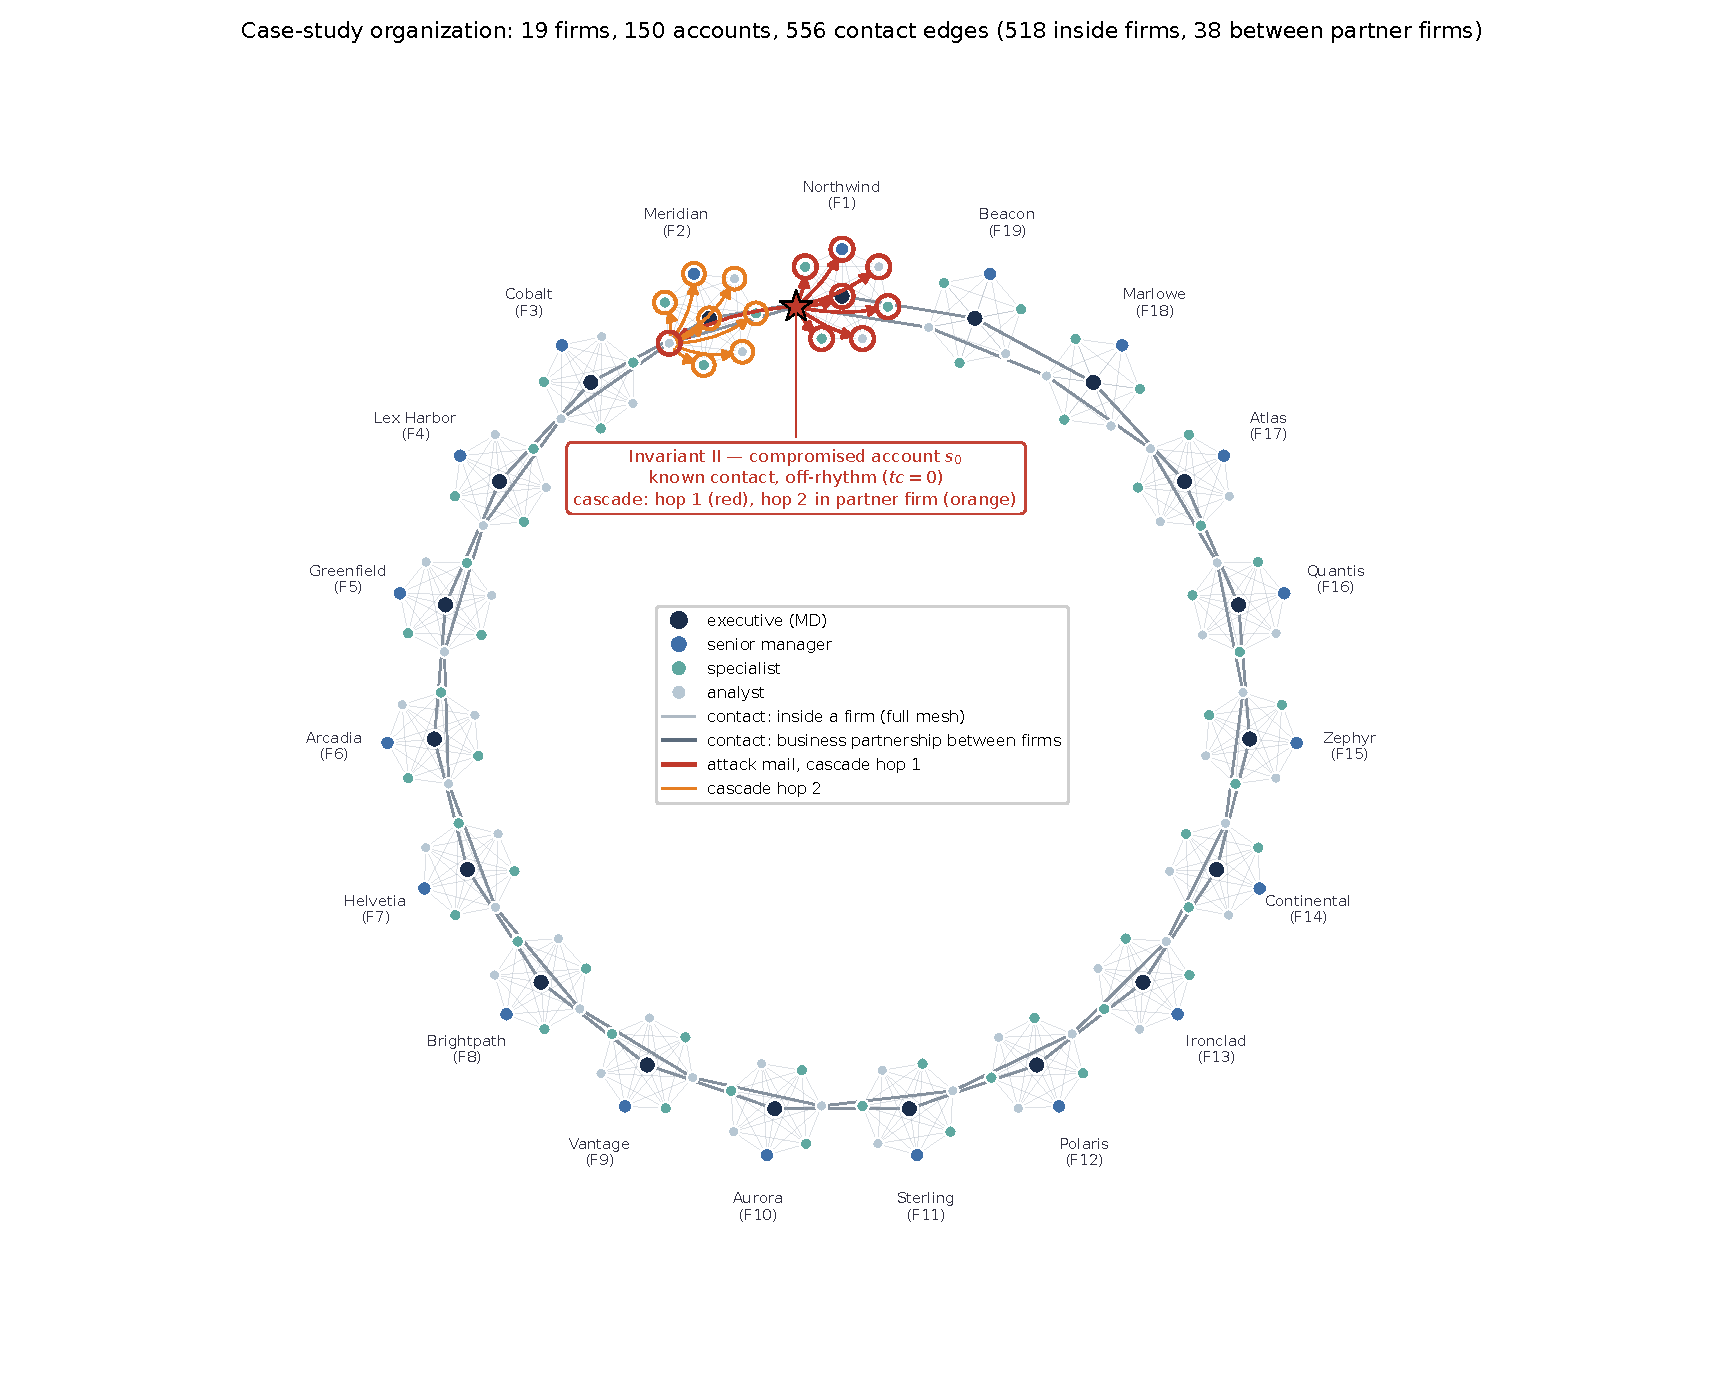
\includegraphics[width=0.95\textwidth]{fig_org_case_study_cascade.pdf}
\caption{Organizacja studyjna z danych populacji paczki
reprodukcyjnej: $19$ firm na pierścieniu partnerstw, $150$ kont
kolorowanych po starszeństwie, warstwa kontaktów ($556$ krawędzi).
Nałożony atak, który detektory muszą wykryć: przejęte konto $s_0$
(gwiazdka), którego poczta poza rytmem kaskadowa się przez własną
firmę (hop~1, czerwony) i przez krawędź partnerską do firmy sąsiedniej
(hop~2, pomarańczowy). Każda wiadomość kaskady pochodzi od realnego
kontaktu; zdradzają ją wyłącznie czas i fala po stronie odbiorców.}
\label{fig:k-casestudy}
\end{figure}

\section{Wyniki: hierarchia detektorów}
\label{sec:k-hierarchia}

Przejęte konto przechodzi każdą relację statyczną, więc sama pozycja
w grafie niesie mało sygnału operacyjnego: GNN statyczny osiąga AUC
$0{,}76$, ale czułość@FPR$1\%$ tylko $0{,}039$
(tab.~\ref{tab:k-detektory}). Sygnał musi więc mieszkać w dynamice.
Tabela~\ref{tab:k-detektory} testuje T1 na kaskadzie domyślnej
i pokazuje wyraźną hierarchię: lokalne cechy 1-hop są bezużyteczne
(AUC $0{,}70$, czułość $\approx 0$), ręczny kontekst kaskadowy
i detektor wolumetryczny COMPA czytają sygnał burstu ($0{,}81$,
odpowiednio $0{,}83$), a temporalny GNN z pamięcią węzłów prowadzi
(AUC $0{,}87$, czułość@FPR$1\%$ $0{,}099$). Przewaga jest temporalna
w sensie ablacyjnym: proste tasowanie porządku czasu cofa model
temporalny do poziomu statycznego ($0{,}87\to0{,}73$; czułość
$0{,}099\to0{,}022$), zgodnie ze stwierdzeniem~\ref{prop:shuffle}.
Wybór architektury znaczy mniej niż paradygmat: TGN-lite wyprzedza
ręczny kontekst we wszystkich ziarnach, a biblioteczny TGN
\citep{rossi2020temporal} dorównuje mu na metryce operacyjnej
(czułość@1\% $0{,}112$ wobec $0{,}078$ TGN-lite przy AUC $0{,}79$
wobec $0{,}85$; 3 ziarna).

\begin{table}[htbp]\centering
\begin{tabular}{lcc}
\toprule
Detektor & AUC & czułość@FPR$1\%$ \\
\midrule
1-hop (tabular)            & $0{,}70$ & $0{,}006$ \\
GNN statyczny              & $0{,}76$ & $0{,}039$ \\
Ręczny kontekst (tab.)     & $0{,}81$ & $0{,}023$ \\
COMPA (wolumetryczny)      & $0{,}83$ & $\mathbf{0{,}232}$ \\
\textbf{GNN temporalny}    & $\mathbf{0{,}87}$ & $0{,}099$ \\
GNN temporalny (tasowany)   & $0{,}73$ & $0{,}022$ \\
\bottomrule
\end{tabular}
\caption{Hierarchia detektorów kaskady na grafie studyjnym (podział
po ofiarach, 5 ziaren; \texttt{exp\_cascade.csv}). Tylko model
temporalny z pamięcią węzłów łączy wysoki AUC z miarą czułości
operacyjnej; COMPA ma wysoką czułość na tym reżimie, bo jej
przyczynowo-zdarzeniowe liczniki widzą rozwijający się burst
(wtw.~\ref{prop:withinbucket}), ale załamuje się w reżimie skrytym
(tab.~\ref{tab:k-stealth}). Tasowanie czasu usuwa przewagę
temporalnego.}
\label{tab:k-detektory}
\end{table}

\section{Wyniki: atakujący skryty}
\label{sec:k-stealth}

Tabela~\ref{tab:k-stealth} jest testem głównym T1: atakujący skryty
łamie detekcję wolumetryczną, ale nie dynamikę. Przy atakującym,
który rozkłada wysyłki w czasie ($K$ nosicieli, jedna wysyłka na
kubełek), detektor wolumetryczny traci sygnał: przy $K{=}1$ jego AUC
spada do $0{,}52$ z czułością $0{,}000$ --- burst nadawczy znika,
więc nie ma żadnego wzrostu per-kubełek, który byle jaka statystyka
wolumetryczna mogłaby zobaczyć --- podczas gdy model temporalny
degraduje łagodniej i trzyma się powyżej losowego (AUC $0{,}59$,
czułość $0{,}049$), czytając falę po stronie odbiorców. Przy
$K\to$blast przewaga wolumetryczna wraca ($0{,}63\to0{,}85$
temporalnego). Wartości na tym wykresie (rysunek~\ref{fig:k-stealth})
czytają się jako krzywa: im skrytszy atak, tym mocniej wolumetryczny
się załamuje.

Sam \emph{bit rytmu} nie wnosi nic w tym harnessie: detektor
rhythm-only trzyma AUC $0{,}50$ na każdym poziomie $K$
(tab.~\ref{tab:k-stealth}), bo --- zgodnie z audytem rytmu
(\texttt{exp\_cascade\_stealth\_tc.csv}) --- poczta poza rytmem
to $75$--$79\%$ zdarzeń ataku \emph{i} $78$--$79\%$ ruchu legalnego:
klasy są po rytmie wymienne. Sygnałem jest fala po stronie
\emph{odbiorców}, nie rytm nadawcy --- co jest empiryczną
koniugacją lematu~\ref{lem:probe}: skoro brzeg czasowy nie
rozdziela klas, marża musi pochodzić ze sprzężenia czasu ze
strukturą grafu.

\begin{table}[htbp]\centering
\begin{tabular}{lcccccc}
\toprule
& \multicolumn{2}{c}{COMPA} & \multicolumn{2}{c}{GNN temporalny} & rhythm-only \\
\cmidrule(lr){2-3}\cmidrule(lr){4-5}\cmidrule(lr){6-6}
Poziom & AUC & cz.@1\% & AUC & cz.@1\% & AUC \\
\midrule
$K{=}1$ (ekstremalnie skryty) & $0{,}52$ & $0{,}000$ & $\mathbf{0{,}59}$ & $\mathbf{0{,}049}$ & $0{,}50$ \\
$K{=}2$ & $0{,}58$ & $0{,}011$ & $\mathbf{0{,}72}$ & $\mathbf{0{,}037}$ & $0{,}51$ \\
$K{=}3$ & $0{,}57$ & $0{,}011$ & $\mathbf{0{,}74}$ & $\mathbf{0{,}049}$ & $0{,}50$ \\
$K{=}5$ & $0{,}61$ & $0{,}031$ & $\mathbf{0{,}76}$ & $\mathbf{0{,}044}$ & $0{,}50$ \\
blast & $0{,}63$ & $0{,}030$ & $\mathbf{0{,}85}$ & $\mathbf{0{,}071}$ & $0{,}54$ \\
\bottomrule
\end{tabular}
\caption{Atakujący skryty na grafie studyjnym ($K$ nosicieli
rozłożonych w czasie; 20 ziaren; \texttt{exp\_cascade\_stealth.csv},
timing deterministyczny). W miarę $K\to1$ detektor wolumetryczny
traci cały sygnał (czułość $0{,}000$), podczas gdy sygnał odbiorczy
modelu temporalnego degraduje łagodniej i trzyma się powyżej
losowego --- główny wynik operacyjny za T1. Sam rytm nadawcy
(rhythm-only) jest bezużyteczny na każdym poziomie.}
\label{tab:k-stealth}
\end{table}

\begin{figure}[htbp]\centering
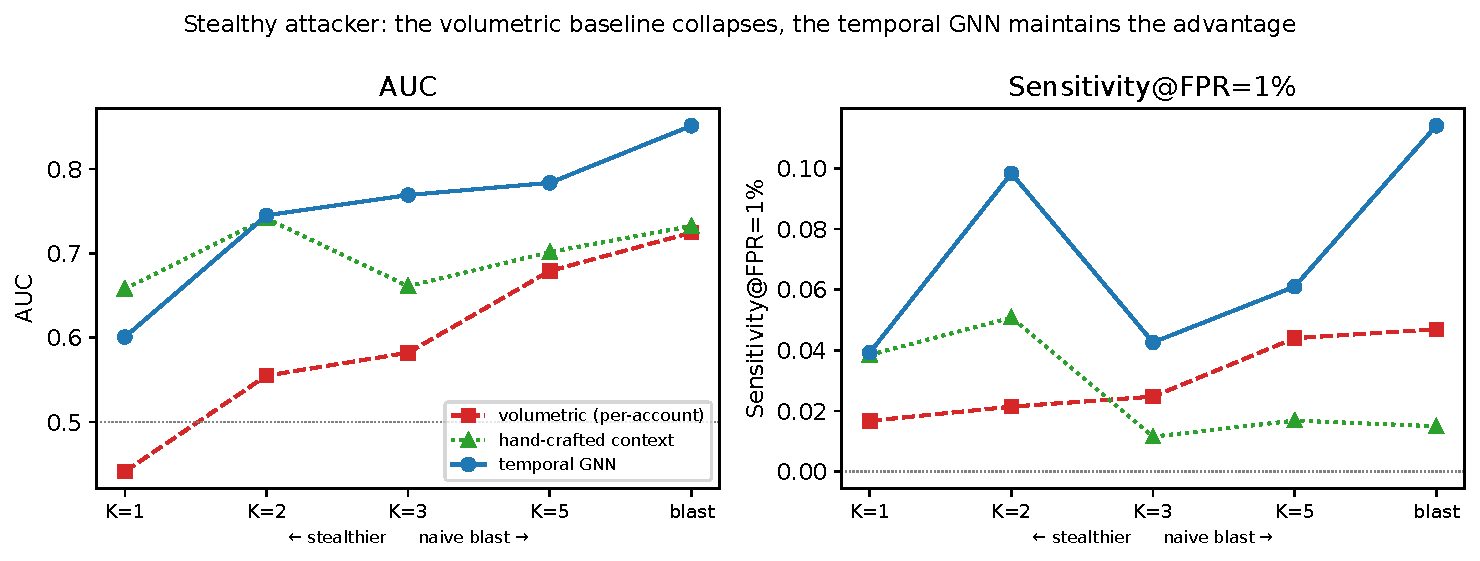
\includegraphics[width=0.9\textwidth]{fig_cascade_stealth.pdf}
\caption{Skrytość a załamanie wolumetryczne: im skrytszy atak
(mniejsze $K$), tym mocniej detektor wolumetryczny się załamuje;
model temporalny degraduje łagodniej dzięki fali po stronie
odbiorców (dane \texttt{exp\_cascade\_stealth.csv}).}
\label{fig:k-stealth}
\end{figure}

\paragraph{Panel baseline'ów.} Tabela~\ref{tab:k-baselines}
stawia ten wynik przeciw dwóm mocnym metodom praktycznym
(harness \texttt{cb}, timing deterministyczny, 20 ziaren). W reżimie
skrytym ręczny kontekst prowadzi przy ekstremalnej skrytości
($K{=}1$: $0{,}77$, przed path-based $0{,}74$ i temporalnym
$0{,}61$), ale traci prowadzenie, gdy tylko kaskada sięga dalej;
path-based degraduje z zasięgiem ($0{,}74\to0{,}65$); a temporalny
GNN jest jedynym detektorem bez reżimu załamania --- w wąskim przedziale
$0{,}61$--$0{,}85$ przez wszystkie poziomy, na prowadzeniu od
$K{=}3$. Ablacja hoppera bez cechy \emph{precursor} pokazuje, że
to właśnie prekursor (odpowiednik świeżości kontekstu ręcznego) niesie
jego sygnał stealth: $0{,}74\to0{,}63$ przy $K{=}1$.

\begin{table}[htbp]\centering\small
\begin{tabular}{lcccccc}
\toprule
Poziom (zasięg) & COMPA & hopper & hopper$\emptyset$prek. & ręczny & temporalny \\
\midrule
$K{=}1$ (11\%) & $0{,}51$ & $0{,}74$ & $0{,}63$ & $\mathbf{0{,}77}$ & $0{,}61$ \\
$K{=}2$ (28\%) & $0{,}58$ & $0{,}70$ & $0{,}63$ & $0{,}69$ & $0{,}68$ \\
$K{=}3$ (46\%) & $0{,}60$ & $0{,}66$ & $0{,}63$ & $0{,}66$ & $\mathbf{0{,}72}$ \\
$K{=}5$ (63\%) & $0{,}64$ & $0{,}65$ & $0{,}64$ & $0{,}68$ & $\mathbf{0{,}77}$ \\
blast (75\%)   & $0{,}70$ & $0{,}82$ & $0{,}79$ & $0{,}75$ & $\mathbf{0{,}85}$ \\
\bottomrule
\end{tabular}
\caption{Panel baseline'ów w reżimie skrytym (AUC, 20 ziaren,
timing deterministyczny; \texttt{cb\_hopper\_stealth.csv}). Ręczny
kontekst prowadzi tylko przy $K{=}1$; hopper degraduje z zasięgiem
(prekursor niesie jego sygnał: $0{,}74\to0{,}63$ po ablacji);
temporalny GNN jest jedynym detektorem bez reżimu załamania.}
\label{tab:k-baselines}
\end{table}

\paragraph{Kontrasty statystyczne.} Wzmocnienie głównego kontrastu
na 20 ziarnach testem Wilcoxona i Cliffa $\delta$
(\texttt{cb\_headline\_contrasts.csv}): sygnał odbiorczy bije detekcję
wolumetryczną istotnie i z dużym efektem (temporalny GNN
$+0{,}115$ AUC, $p<0{,}001$, $\delta=0{,}98$; w protokole benign
empirycznym $+0{,}113$, $\delta=0{,}99$), podczas gdy temporalny
GNN \emph{nie} bije istotnie kontekstu ręcznego ($+0{,}021$,
$p=0{,}19$; w protokole empirycznym $+0{,}002$, $p=0{,}93$):
sygnał odbiorczy czytają równie dobrze model nauczony i cechy
ręczne. Załamanie wolumetryczne nie jest artefaktem strojenia:
COMPA nie ma okna ani progu do strojenia --- jej trzy cechy to
liczniki na obserwowanym strumieniu karmione tym samym learnerem
co każda inna metoda tabularna --- więc załamanie jest własnością
modelu ataku: jedna wysyłka na kubełek nie zostawia żadnego
per-kubełkowego wzrostu dla żadnej statystyki wolumetrycznej.

\section{Wyniki: granice modelu zagrożeń}
\label{sec:k-granice}

Tabela~\ref{tab:k-fanout} wyznacza mierzalną dolną granicę tego, co
detektory widzą (RQ2). W reżimie chirurgicznym ($p_{\mathrm{inf}}=0$,
bez jakiejkolwiek propagacji) atak na jednego odbiorcę jest
niewidoczny dla każdego detektora (AUC $0{,}48$--$0{,}53$): sygnał
wymaga fan-outu $\ge2$. Blok pokazuje też coś mniej oczywistego:
\emph{sama propagacja nie jest potrzebna} --- przy
$p_{\mathrm{inf}}=0$ i fan-oucie $\ge2$ atak jest wykrywany zarówno
przez wolumetryczny ($0{,}68$--$0{,}83$), jak i temporalny
($0{,}75$--$0{,}94$), bo kilka odbiorców w jednym otoczeniu
trafionych naraz już tworzy zsynchronizowany burst nadawczy i falę
odbiorczą. Sygnał wymaga fan-outu, nie kaskady; kaskada jest ważna,
bo to ona pozwala atakującemu skrytemu dotrzeć do wielu ofiar
\emph{bez} takiego burstu.

\begin{table}[htbp]\centering
\begin{tabular}{lcccc}
\toprule
Fan-out & COMPA & hopper & ręczny & temporalny \\
\midrule
$1$ (pojedynczy odbiorca) & $0{,}50$ & $0{,}48$ & $0{,}53$ & $0{,}51$ \\
$2$ & $0{,}68$ & $0{,}50$ & $0{,}55$ & $0{,}75$ \\
$3$ & $0{,}76$ & $0{,}52$ & $0{,}54$ & $0{,}85$ \\
$5$ & $\mathbf{0{,}83}$ & $0{,}50$ & $0{,}52$ & $\mathbf{0{,}94}$ \\
\bottomrule
\end{tabular}
\caption{Atak chirurgiczny bez propagacji ($p_{\mathrm{inf}}=0$),
po fan-oucie (AUC, 20 ziaren; \texttt{cb\_surgical\_fanout.csv}):
atak na jednego odbiorcę jest punktem ślepym każdego detektora;
sygnał wymaga fan-outu $\ge2$, a nie propagacji.}
\label{tab:k-fanout}
\end{table}

\section{Wyniki: stabilność i generalizacja indukcyjna}
\label{sec:k-stabilnosc}

Trzy kontrole ograniczają odczyt T1. \emph{Sweep parametrów kaskady}
(\texttt{exp\_cascade\_sweep.csv}): hierarchia temporalna trzyma się
w całym zakresie $p_{\mathrm{inf}}\in[0{,}05,0{,}5]$ (GNN temporalny
AUC $0{,}87$--$0{,}97$); sygnał odbiorczy nie znika przy realistycznie
niskiej zakaźności, choć przy bardzo niskim $p_{\mathrm{inf}}$
detektor wolumetryczny odzyskuje wysoką czułość operacyjną
(r@1\% $0{,}59$ przy $p_{\mathrm{inf}}{=}0{,}05$), bo rzadsze
kaskady zostawiają czystszą cechę nowości wolumetrycznej ---
zależność, którą jawnie odnotowujemy jako niemonotoniczność w
p~$p_{\mathrm{inf}}$. \emph{Szum etykiet} (\texttt{cb\_labelnoise.csv},
tab.~\ref{tab:k-noise}): odwracanie rosnącej frakcji etykiet
treningowych degraduje najszybciej model nauczony (temporalny
$0{,}72\to0{,}59$ przy $20\%$ szumu; COMPA tylko $0{,}60\to0{,}57$):
przy realistycznym szumie etykiet przewaga modelu nauczonego się
kurczy. \emph{Podział indukcyjny po organizacjach}
(\texttt{exp\_cascade\_org.csv}; skale 240/1600 kont w
\texttt{exp\_cascade\_scale*.csv}): na firmach niewidzianych
w treningu przewagę AUC przejmuje detektor wolumetryczny
($0{,}83$ wobec $0{,}72$ temporalnego), zgodnie z wnioskiem
indukcyjnym z rozdziału formalnego: cechy wolumetryczne
transferują się najlepiej, sygnał odbiorczy degraduje między
organizacjami; model temporalny zachowuje jednak czułość
operacyjną powyżej swojego poziomu losowego (r@1\% $0{,}086$,
najwyższą poza COMPA). Detektor temporalny jest więc lepszym
detektorem \emph{operacyjnym} w rozkładzie, niż rankerem między
organizacjami --- w skalach, które badamy.

\begin{table}[htbp]\centering
\begin{tabular}{lcccc}
\toprule
Szum etykiet & COMPA & hopper & ręczny & temporalny \\
\midrule
$0\%$   & $0{,}60$ & $0{,}66$ & $0{,}66$ & $\mathbf{0{,}72}$ \\
$5\%$   & $0{,}59$ & $0{,}66$ & $0{,}65$ & $\mathbf{0{,}68}$ \\
$10\%$  & $0{,}58$ & $0{,}65$ & $0{,}64$ & $\mathbf{0{,}64}$ \\
$20\%$  & $0{,}57$ & $\mathbf{0{,}63}$ & $0{,}61$ & $0{,}59$ \\
\bottomrule
\end{tabular}
\caption{Szum etykiet treningowych (AUC, 20 ziaren;
\texttt{cb\_labelnoise.csv}): model nauczony degraduje najszybciej
($0{,}72\to0{,}59$ przy $20\%$), baseline wolumetryczny najwolniej.}
\label{tab:k-noise}
\end{table}

\section{Wyniki: walidacja na realnych grafach komunikacji}
\label{sec:k-realne}

Realne grafy (Enron \citep{klimt2004enron}, dwa grafy SNAP:
\texttt{email-Eu-core} \citep{paranjape2017motifs} i
\texttt{CollegeMsg} \citep{panzarasa2009patterns}) służą walidacji
mechanizmu tam, gdzie struktura i rytmy są prawdziwe. Etykiety ataku
to kontrolowane iniekcje pod projektem dopasowanym: legalny ruch
i atak mają ten sam rozkład końców i stopni, różnią się wyłącznie
wzorcem czasowym --- więc różnice wyników są przypisywalne dynamice.
Sonda predyktywności sprawdza dwie rzeczy: czy jakościowa
hierarchia detektorów odtwarza się na każdej topologii, i czy
kontrast główny (sygnał odbiorczy vs wolumetryczny) zachowuje
kierunek.

\paragraph{Enron ($\sim\!1970$ kont, 8 ziaren).}
Tabela~\ref{tab:k-enron}, blok (a): w reżimie blast hierarchia
z grafu studyjnego odtwarza się --- 1-hop $0{,}65$, ręczny kontekst
$0{,}74$, COMPA $0{,}87$ (czułość $0{,}19$), temporalny $0{,}80$,
a tasowanie czasu sprowadza temporalny do poziomu ręcznego
kontekstu ($0{,}74$). W reżimie skrytym --- blok (b) --- COMPA
załamuje się (AUC $0{,}69$, czułość $0{,}000$), podczas gdy
sygnał odbiorczy trzyma: temporalny $0{,}85$ (czułość $0{,}22$),
ręczny kontekst $0{,}87$ (czułość $0{,}21$). Pod timingiem
empirycznym (odstępy z prawdziwych nadawców, tw.~\ref{thm:injection})
temporalny utrzymuje marżę $0{,}77$ nad poziomem wolumetrycznym.
Zgodnie ze stwierdzeniem~\ref{prop:withinbucket} asymetria
mechanizmu jest mierzalna bezpośrednio (\texttt{exp\_blast\_inversion.csv}):
na Enronie odsetek zdarzeń ataku, których fala otoczenia przypada
ściśle w przeszłych kubełkach, wynosi $0{,}21$--$0{,}25$, podczas
gdy $0{,}58$--$0{,}64$ ofiar jest trafionych wielokrotnie \emph{w tym
samym kubełku} --- dokładnie ta asymetria jest mechanizmem inwersji
blast: detektory odbiorcze przegrywają tam, gdzie
wewnątrzkubełkowe liczniki wolumetryczne wygrywają.

\begin{table}[htbp]\centering\small
\begin{tabular}{llcc}
\toprule
Reżim & Detektor & AUC & czułość@1\% \\
\midrule
\multicolumn{4}{@{}l}{\emph{(a) blast --- kaskada naiwna, projekt dopasowany, 8 ziaren}} \\
blast & 1-hop (tabular)          & $0{,}65$ & $0{,}019$ \\
      & Ręczny kontekst (tab.)    & $0{,}74$ & $0{,}031$ \\
      & COMPA (wolumetryczny)     & $\mathbf{0{,}87}$ & $\mathbf{0{,}192}$ \\
      & GNN temporalny            & $0{,}80$ & $0{,}054$ \\
      & GNN temporalny (tasowany)& $0{,}74$ & $0{,}048$ \\
\midrule
\multicolumn{4}{@{}l}{\emph{(b) stealthy --- atakujący skryty, 8 ziaren}} \\
stealthy & 1-hop (tabular)        & $0{,}61$ & $0{,}019$ \\
      & Ręczny kontekst (tab.)    & $\mathbf{0{,}87}$ & $\mathbf{0{,}213}$ \\
      & COMPA (wolumetryczny)     & $0{,}69$ & $0{,}000$ \\
      & \textbf{GNN temporalny}   & $0{,}85$ & $0{,}215$ \\
      & GNN temporalny (tasowany) & $0{,}76$ & $0{,}081$ \\
\bottomrule
\end{tabular}
\caption{Replikacja na realnym grafie kontaktów Enron
($\sim\!1970$ kont; \texttt{exp\_cascade\_enron.csv}). (a)~W blast
hierarchia studyjna odtwarza się, a tasowanie czasu sprowadza model
temporalny do poziomu cech ręcznych. (b)~Pod atakiem skrytym
wolumetryczny traci cały sygnał operacyjny (czułość $0{,}000$),
a sygnał odbiorczy trzyma czułość $\approx0{,}21$.}
\label{tab:k-enron}
\end{table}

\paragraph{SNAP (3 ziarna).}
Tabela~\ref{tab:k-snap}: przejście reżimowe replikuje się w kierunku
na obu grafach. Przeciw naiwnemu blastowi wygrywa detektor
wolumetryczny ($0{,}83$ na obu grafach; jego
przyczynowo-zdarzeniowe liczniki widzą burst, którego oknom
strictly-past detektorów odbiorczych brakuje na rzadkiej
topologii --- CollegeMsg ma klastrowanie $0{,}14$ wobec $0{,}45$
\texttt{email-Eu-core}), podczas gdy temporalny osiąga $0{,}63$.
Przeciw atakującemu skrytemu wolumetryczny spada ($0{,}66$/$0{,}63$),
a sygnał odbiorczy trzyma przewagę: temporalny $0{,}81$/$0{,}82$,
ręczny kontekst $0{,}86$/$0{,}83$ (czułości $0{,}08$--$0{,}12$ przy
$0{,}00$ wolumetrycznego). Sonda predyktywności jest więc
pozytywna w sensie reżimowym: na każdym z trzech realnych grafów
wolumetryczny wygrywa blast i załamuje się pod skrytością,
a sygnał odbiorczy trzyma się wyżej --- przenoszalny jest kontrast
reżimowy, nie pełny ranking detektorów. Przy 3--8 ziarnach na graf
test per-graf Wilcoxona nie osiąga konwencjonalnej istotności
(dwustronne $p\ge0{,}25$ przy $n{=}3$), więc replikacje realne
czytamy jako potwierdzenia kierunkowe.

\begin{table}[htbp]\centering\small
\begin{tabular}{llccc}
\toprule
Graf (reżim) & Detektor & AUC & czułość@1\% \\
\midrule
\texttt{email-Eu-core} (blast) & COMPA / temporalny & $\mathbf{0{,}83}$ / $0{,}63$ & $\mathbf{0{,}121}$ / $0{,}021$ \\
\texttt{email-Eu-core} (skryty) & COMPA / temporalny & $0{,}66$ / $\mathbf{0{,}81}$ & $0{,}002$ / $\mathbf{0{,}075}$ \\
\texttt{CollegeMsg} (blast) & COMPA / temporalny & $\mathbf{0{,}83}$ / $0{,}64$ & $\mathbf{0{,}112}$ / $0{,}027$ \\
\texttt{CollegeMsg} (skryty) & COMPA / temporalny & $0{,}63$ / $\mathbf{0{,}82}$ & $0{,}005$ / $\mathbf{0{,}109}$ \\
\bottomrule
\end{tabular}
\caption{Replikacja reżimowa na dwóch grafach SNAP (3 ziarna;
\texttt{exp\_cascade\_realgraphs.csv}): wolumetryczny wygrywa
naiwny blast i załamuje się pod atakiem skrytym; sygnał odbiorczy
temporalnego zachowuje przewagę w reżimie skrytym na obu
topologiach (czułości: patrz tekst; ręczny kontekst $0{,}86$/$0{,}83$).}
\label{tab:k-snap}
\end{table}

\section{Rygor: co znaczy, że detektor działa}
\label{sec:k-rygor}

\paragraph{Arytmetyka bazy.} Czułość przy danym FPR jest niezależna
od prewalencji, ale precyzja spada, gdy atak jest rzadki. Z
arytmetyki Bayesa (stw. o~bazie, rozdz.~\ref{rozd:formalny}): przy
punkcie pracy (czułość $r{=}0{,}10$, FPR $\alpha{=}1\%$) i realnej
prewalencji $1{:}10^4$ każde wykryte zdarzenie ataku niesie
$\sim\!10^3$ fałszywych alarmów; w reżimie skrytym, gdzie
$r\approx0{,}03$, na każde wykrycie przypada $\sim\!3300$ fałszywych
alarmów. Nasz punkt pracy ($\alpha=10^{-2}$) jest przy tym
\emph{liberalny} wobec progu operacyjnego realnej poczty
($<\!4$ FP na milion, \citealp{ho2019detecting}; różnica trzech
rzędów wielkości). Konsekwencja: przy realnej prewalencji detektory
tej klasy --- i każdy detektor o podobnej krzywej ROC --- są
instrumentem triażu i rankingu dla analityków SOC, nie autonomiczną
blokadą; wkład rozdziału leży w sygnale, mechanizmie i metodologii,
nie w produkcie.

\paragraph{Operacyjna definicja skuteczności.} Metoda operacyjna
spełnia standard rozdziału formalnego: jej przewaga znika pod
kontrolą tasowania czasu (test pozytywny: znika), przenosi się
na realne topologie w sensie kontrastu reżimowego (sonda
predyktywności pozytywna), jest mierzona w niskim FPR z jawną
prewalencją, a jej granice --- punkt ślepy fan-out 1, szum etykiet,
degradacja indukcyjna sygnału odbiorczego --- są wypowiedziane.
Przy tym standardzie „98\% na benchmarku masowym" nie mówi nic
o lateral phishingu; liczy się czułość na ogon ukierunkowany,
z wyznaczoną podłogą i progmem jeszcze rzędy wielkości odległym.

\section{Podsumowanie rozdziału}
\label{sec:k-podsumowanie}

\paragraph{RQ1 (sygnał).} Przejęte konto zgodne z każdą statyczną
relacją jest wykrywalne z dynamiki kaskady: fala po stronie
odbiorców, czytana przez model temporalny z pamięcią węzłów,
degraduje pod atakującym skrytym łagodniej i trzyma się powyżej
losowego, podczas gdy detekcja wolumetryczna traci cały sygnał
operacyjny (czułość $0{,}000$ przy $K{=}1$); przewaga jest temporalna
w sensie ablacyjnym (znika pod tasowaniem) i przenosi się
kierunkowo na trzy realne grafy komunikacji. Formalnie: sygnał
mieszka w sprzężeniu czasu ze strukturą grafu, nie w brzegu
czasowym (lemat~\ref{lem:probe}: rhythm-only $=0{,}50$), a jego
widoczność ogranicza ślepota wewnątrzkubełkowa dokładnie tak,
jak opisuje stwierdzenie~\ref{prop:withinbucket}
(\texttt{exp\_blast\_inversion.csv}: $0{,}21$--$0{,}25$ trafień
wczesniejszych wobec $0{,}58$--$0{,}64$ wielokrotnych
wewnątrzkubełkowych).

\paragraph{RQ2 (granice).} Sygnał wymaga fan-outu $\ge2$; atak
chirurgiczny na jednego odbiorcę jest punktem ślepym każdego
detektora. Przewaga degraduje łagodnie ze skalą i kurczy się pod
szumem etykiet (model nauczony degraduje najszybciej:
$0{,}72\to0{,}59$ przy $20\%$); między organizacjami najlepiej
transferują się cechy wolumetryczne, ale model temporalny zachowuje
czułość operacyjną. Przy realnej prewalencji detektory są
instrumentem triażu ($\sim\!10^3$ fałszywych alarmów na wykrycie).

Rozdział obronił tezę dla kanału lateral. Komplementarny kanał ---
impersonacja zewnętrzna roli/autorytetu, wymagająca wiedzy
wykraczającej poza graf komunikacji --- jest przedmiotem
rozdziału~\ref{rozd:multipleks}.

% =====================================================================
% ROZDZIAŁ 5 — Spear phishing jako naruszenie grafu wiedzy domenowej
% (na bazie artykułu B, IEEE; liczby wprost z code/results/*.csv)
% =====================================================================
\chapter{Spear phishing jako naruszenie grafu wiedzy domenowej}
\label{rozd:multipleks}

\section{Teza cząstkowa i plan rozdziału}
\label{sec:m-teza}

Ten rozdział rozwija drugą połowę tezy T1 oraz metodologiczną stronę
T2: impersonacja zewnętrzna (spear phishing w reżimie BEC) odnosi
sukces, \emph{respektując} wiedzę domenową ofiary --- nadawca podszywa
się pod znaną rolę lub autorytet, a treść czyta się jak normalna
poczta. Teza: sygnał nie leży w treści, lecz w jej
\emph{niespójności} z grafem wiedzy domenowej organizacji, który
modelujemy jako multiplex relacji na jednym zbiorze kont --- kontakty,
hierarchia, kompetencje, publiczny ślad (OSINT), platformy, rutyny
oraz rytm czasowy. Prawdziwa relacja jest spójna w wielu warstwach
naraz; impersonacja pojawia się w jednej warstwie, a przeczy
pozostałym. Rozdział odpowiada na RQ3 (niespójność międzywarstwowa
jako sygnał) i RQ4 (narażenie i granice), a przy okazji dostarcza
empirycznej instancji twierdzenia o look-ahead
(tw.~\ref{thm:lookahead}): \emph{pułapki wycieku rytmu}.

Plan: sekcja~\ref{sec:m-model} formalizuje graf wiedzy domenowej
i niezmiennik niespójności międzywarstwowej; sekcja~\ref{sec:m-metoda}
--- detektory, kontrolę tasowania i miarę narażenia;
sekcja~\ref{sec:m-studium} opisuje organizację studyjną i jej warstwy;
wyniki zajmują sekcje
\ref{sec:m-mechanizm}--\ref{sec:m-tresc}; sekcja
\ref{sec:m-podsumowanie} podsumowuje odpowiedzi na RQ3--RQ4. Zakres
jest wyznaczony z góry: warstwy OSINT są syntetyczne (także na
realnym grafie), więc rozdział --- jak cały artykuł B --- dowodzi
mechanizmu i praktyki ewaluacyjnej, nie detekcji realnych intruzji.
Komplementarny kanał (przejęte konto wewnętrzne propagujące kaskadę)
używa wyłącznie warstwy kontaktów i rytmu i był przedmiotem
rozdziału~\ref{rozd:kaskada}.

\section{Model: graf wiedzy domenowej}
\label{sec:m-model}

\begin{definition}[Graf wiedzy domenowej]
\label{def:m-dkg}
\emph{Graf wiedzy domenowej} to
$\mathcal{G}=(V,\{E_L\}_{L\in\mathcal{L}},\{w_L\},\tau)$, gdzie $V$
to zbiór kont, $\mathcal{L}$ --- zbiór relacyjnych \emph{warstw} na
tym \emph{samym} $V$ (kontakty, hierarchia, domena; warstwy OSINT:
kompetencje, publiczny ślad, platformy, wydarzenia, rutyny,
preteksty), $w_L\in(0,1]$ --- waga ufności warstwy, a
$\tau\colon V\to\mathcal{T}$ przypisuje nadawcom \emph{rytm czasowy}
(zbiór aktywnych okien).
\end{definition}

Dwa skalary podsumowują parę nadawca--ofiara. \emph{Pokrycie wiedzy
domenowej} waży warstwy, w których para ko-występuje,
\begin{equation}
C(s,v)\;=\;\sum_{L\in\mathcal{L}} w_L\,\mathbf{1}\!\left[(s,v)\in E_L\right],
\label{eq:m-coverage}
\end{equation}
a \emph{spójność czasowa} testuje, czy wiadomość przychodzi
w rytmie nadawcy, $tc(s,v,t)=\mathbf{1}[t\in\tau(s)]$. Rytm liczony
z \emph{pełnej historii} jest nieprzyczynową cechą w sensie
definicji~\ref{def:causal-feature} --- to właśnie jest mechanizm
pułapki z sekcji~\ref{sec:m-enron} i tw.~\ref{thm:lookahead}.

\paragraph{Model zagrożeń.} Celem atakującego jest dostarczenie
ofiarami $v$ wiadomości sklasyfikowanej jako legalna. W
impersonacji zewnętrznej $s$ podszywa się pod rolę lub autorytet,
dając wrażenie wysokiego $C(s,v)$, nie mając realnego pokrycia
w części warstw (niska spójność strukturalna), ewentualnie
\emph{fabrykując} krawędzie OSINT. Sfabrykowanie śladu publicznego
jest tanie, ale samo w sobie nie tworzy spójności wielowarstwowej ---
to jest sygnał; fabrykację traktujemy formalnie (stw.~\ref{prop:fab})
i empirycznie (sweep, sekcja~\ref{sec:m-fabrykacja}). Przejęte konto
wewnętrzne to przypadek komplementarny: $C(s,v)$ wysokie, lecz
$tc=0$. Poza modelem pozostaje adaptacyjny przeciwnik z pełną
wiedzą o grafie.

\paragraph{Niezmiennik: niespójność międzywarstwowa.}
Legalny nowy nadawca siedzi poza warstwą kontaktów ofiary, ale
\emph{na} którejś warstwie OSINT --- i ta spójność go usprawiedliwia;
impersonator siedzi poza każdą warstwą albo na jednej, którą
pozostałe przeczą. Detektor działa na wektorze przynależności
warstwowych i jego (nie)spójności, pomijając treść. Niezmiennik jest
testowalny ablacją: tasowanie przynależności warstwowych i rytmu
niszczy strukturę, na której polega (kontrola tasuje też kontakty
i rytm, więc \emph{ogranicza}, a nie izoluje wkład międzywarstwowy
--- stw.~\ref{prop:shuffle}).

\section{Metoda: detektory, kontrola, narażenie}
\label{sec:m-metoda}

\paragraph{Detektory.} Dla pary nadawca--ofiara porównujemy trzy
zestawy cech o rosnącej strukturze, zawsze z gradient boostingiem:
\emph{kontakty} (tylko warstwa kontaktów), \emph{multiplex
statyczny} (dodane warstwy OSINT) oraz \emph{multiplex + rytm}
(dodana cecha $tc$). Cechy kodują przynależność warstwową i czas,
nigdy tożsamość, więc każdy detektor jest indykcyjny. Kontrola
tasowania permutuje przynależności warstwowe i rytm: jeśli sygnał
jest rzeczywistą spójnością międzywarstwową, kontrola musi cofnąć
przewagę do losowej. Kontrolę stosujemy w dwóch wariantach ---
pełnym (tasowane wszystkie cechy) i \emph{tylko-OSINT} (kontakty
i rytm nietknięte) --- bo pełna kontrola miesza sygnał warstwowy
z sygnałem kontaktów i rytmu.

\paragraph{Zdarzenia i podziały.} Zdarzenie to trójka (nadawca,
ofiara, kubełek) z etykietą i szumem po obu stronach. Po stronie
legalnej trzy rodzaje nadawców: znany kontakt piszący w rytmie;
\emph{nowy-OSINT} --- poza kontaktami ofiary, ale współdzielący
z nią warstwę OSINT; oraz nadawca \emph{zimny} --- poza każdą
warstwą, którego żaden detektor relacyjny nie może unieważnić
(podłoga fałszywych alarmów). Po stronie ataku dwa kanały:
zewnętrzne BEC (poza wszystkimi warstwami, poza rytmem) i przejęty
znany kontakt piszący poza rytmem. Ofiary testowe są rozłączne od
treningowych (stw.~\ref{prop:split}); liczby główównie uśrednione
po 20 ziarnach; metryka główna to czułość@FPR$1\%$ z AUC obok.

\begin{definition}[Narażenie detektorowo-relatywne]
\label{def:m-susc}
\emph{Narażeniem} węzła $v$ względem detektora $D$ przy ustalonym
FPR, dla kanału ataku $c$, jest oczekiwana stopa chybień ataków
tego kanału wymierzonych w $v$:
$\mathrm{Susc}_{D,c}(v)=\E_{s\in\mathcal{A}_c(v)}
\big[1-\Pr[D\ \text{wykrywa}\ (s\!\to\!v)]\big]$,
gdzie $\mathcal{A}_c(v)$ to zbiór atakujących $v$ w kanale $c$.
\end{definition}

$\mathrm{Susc}_D$ mierzy \emph{rezydualne} narażenie, które detektor
zostawia --- nie ludzką podatność ofiary \citep{halevi2015spearphishing,
butavicius2022why}; wyższe wartości znaczą \emph{bardziej} narażone.
Nie enumerujemy $\mathcal{A}_c(v)$; estymator plug-in grupowy
z sekcji~\ref{sec:m-susc} liczy $\mathrm{Susc} = 1 -
\text{czułość@1\%}$ per kanał i starszeństwo, z bootstrapowymi
przedziałami ufności po ziarnach.

\section{Studium przypadku: organizacja i warstwy}
\label{sec:m-studium}

Organizacja studyjna to ten sam ekosystem co w
rozdziale~\ref{rozd:kaskada}: $19$ firm z różnych sektorów, $N{=}150$
kont, $556$ krawędzi kontaktów, generacja \emph{graph-first}
(rysunek~\ref{fig:m-casestudy}). Każda persona jest rekordem
o ustalonym schemacie ośmiu kategorii (tożsamość zawodowa,
relacje, kompetencje, publiczny ślad, kanały kontaktu, kontekst
czasowy, profil perswazji, rutynowa komunikacja z wiarygodnymi
pretekstami) --- i te kategorie są dokładnie materiałem OSINT
dostępnym dla atakującego; każda mapuje się na co najwyżej jedną
warstwę (tab.~\ref{tab:m-warstwy}). Dwie persony łączy krawędź
w warstwie, gdy współdzielą konkretną, publicznie obserwowalną
wartość pola; wartości generyczne są odfiltrowane. Tydzień:
$T{=}28$ kubełków sześciogodzinnych; rytm to $6$ aktywnych
kubełków na personę; $15\%$ legalnej poczty poza rytmem, $25\%$
ataków w mimikrii rytmu.

\begin{figure}[htbp]\centering
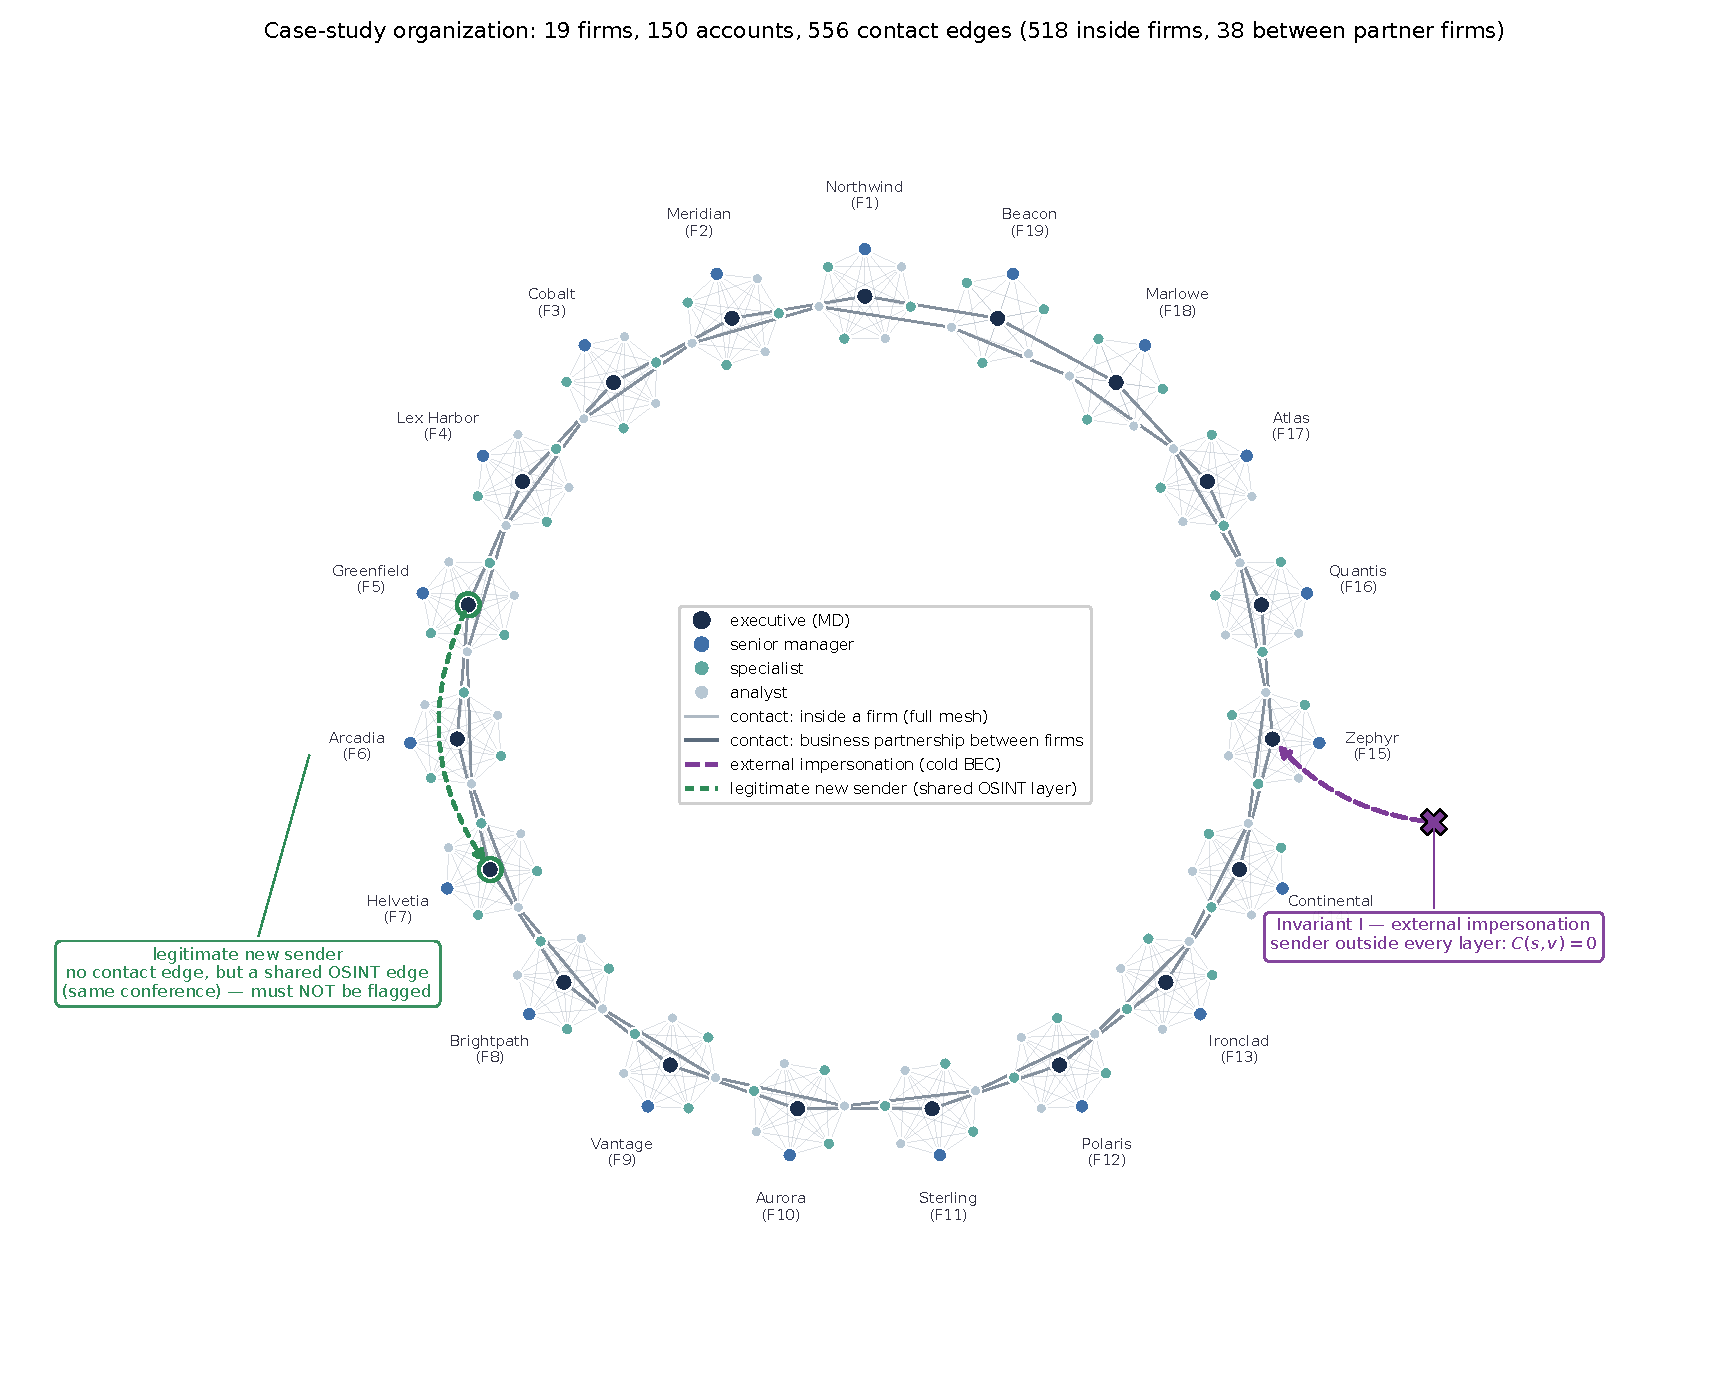
\includegraphics[width=0.95\textwidth]{fig_org_case_study_inv1.pdf}
\caption{Organizacja studyjna z danych populacji: $19$ firm na
pierścieniu partnerstw, $150$ kont kolorowanych po starszeństwie,
warstwa kontaktów ($556$ krawędzi). Nałożone dwa przypadki, które
detektor musi rozdzielić: impersonacja zewnętrzna spoza każdej
warstwy ($C(s,v){=}0$) oraz legalny nowy nadawca podłączony wyłącznie
przez współdzieloną warstwę OSINT (ta sama konferencja) --- który
nie może zostać oflagowany.}
\label{fig:m-casestudy}
\end{figure}

\begin{table}[htbp]\centering\small
\begin{tabular}{llcc}
\toprule
Warstwa & Krawędź (współdzielony fakt) & $w_L$ & \#krawędzi \\
\midrule
Kontakty       & nadawca pisał do odbiorcy        & $1{,}0$ & $556$ \\
Hierarchia     & ta sama firma                    & $0{,}9$ & $518$ \\
Domena         & ta sama domena pocztowa          & $0{,}8$ & $538$ \\
OSINT: konferencje & współdzielona konferencja    & $0{,}6$ & $167$ \\
OSINT: certyfikaty & współdzielony certyfikat     & $0{,}6$ & $389$ \\
OSINT: umiejętności & współdzielona umiejętność   & $0{,}5$ & $1144$ \\
OSINT: rutyna  & wsp. wzorzec komunikacji         & $0{,}4$ & $397$ \\
OSINT: wydarzenia & wsp. wydarzenie                & $0{,}4$ & $134$ \\
OSINT: platformy & wsp. platforma/handle           & $0{,}4$ & $534$ \\
OSINT: preteksty & wsp. wiarygodny pretekst        & $0{,}3$ & $159$ \\
OSINT: zainteresowania & pokrywające się zainteresowania & $0{,}3$ & $53$ \\
Czasowa        & ko-aktywność w tych samych godzinach & $0{,}5$ & $2528$ \\
\bottomrule
\end{tabular}
\caption{Warstwy multipleksu studyjnego: semantyka krawędzi, waga
ufności $w_L$ (równ.~\eqref{eq:m-coverage}), liczba krawędzi
(paczka reprodukcyjna, dane warstw).}
\label{tab:m-warstwy}
\end{table}

\section{Wyniki: niespójność międzywarstwowa jako mechanizm}
\label{sec:m-mechanizm}

Tabela~\ref{tab:m-inv1} testuje niezmiennik na dwóch przypadkach
z rysunku~\ref{fig:m-casestudy}. Fuzja warstw wiedzy domenowej
z rytmem podnosi AUC z $0{,}70$ (same kontakty) do $0{,}88$, podczas
gdy kontrola tasowania spada do losowego ($0{,}51$): przewaga
pochodzi ze struktury warstw i rytmu, nie z pojemności cech.
Najbardziej uderzająca jest strona fałszywych alarmów: detektor
kontaktowy flaguje \emph{każdego} legalnego nowego nadawcę
(FP $1{,}00$), multiplex --- \emph{żadnego} ($0{,}00$): pokrycie
OSINT ratuje legalnego nadawcę, który współdzieli z ofiarą
obserwowalny fakt.

Stwierdzamy jedną cyrkularność jawnie. W modelu zdarzeń legalny
nowy nadawca jest \emph{zdefiniowany} jako konto siedzące na
jakiejś warstwie OSINT ofiary, więc część likwidacji fałszywych
alarmów jest prawdziwa z konstrukcji: detektor kontaktowy nie może
tej warstwy zobaczyć, multiplex może. Netautologiczna jest reszta
dowodu: kontrola tasowania, która zachowuje brzegowe rozkłady cech
i spada do losowego ($0{,}51$, \emph{poniżej} samych kontaktów) ---
zysk zależy więc od rzeczywistej wspólnej struktury cech; sweep
fabrykacji, w którym fałszywe ślady erodują przewagę stopniowo,
nie skokowo (sekcja~\ref{sec:m-fabrykacja}); oraz wynik Enronu
(sekcja~\ref{sec:m-enron}), gdzie każda warstwa jest zbudowana
z prawdziwych nagłówków.

\begin{table}[htbp]\centering
\begin{tabular}{lcc}
\toprule
Model & AUC & FP na nowych nadawcach \\
\midrule
Kontakty               & $0{,}70$ & $1{,}00$ \\
Multiplex + rytm       & $\mathbf{0{,}88}$ & $\mathbf{0{,}00$} \\
Multiplex (tasowany)   & $0{,}51$ & --- \\
\bottomrule
\end{tabular}
\caption{Niespójność międzywarstwowa na grafie studyjnym (20 ziaren;
\texttt{exp\_multiplex.csv}: konfiguracja domyślna). Fuzja warstw
z rytmem podnosi AUC z $0{,}697$ do $0{,}875$ i likwiduje każdy
fałszywy alarm na legalnych nowych nadawcach; kontrola tasowania
spada do $0{,}505$.}
\label{tab:m-inv1}
\end{table}

Sygnał to zwięzła \emph{spójność}, nie pojemność: cztery jawne
miary spójności (pokrycie OSINT; znany nadawca poza rytmem; nowy
nadawca na OSINT; całkowicie poza grafem) dorównują pełnej
konkatenacji per-warstwa (\texttt{exp\_consistency.csv}: modele
liniowe $0{,}860$ wobec $0{,}840$; drzewa $0{,}860$ wobec $0{,}858$),
a ich wartość leży w wyjaśnialności i wdrożeniu single-query,
nie w czułości (recall).

\paragraph{Ablacja: co niesie sygnał.}
Rysunek~\ref{fig:m-ablation} pokazuje, skąd sygnał pochodzi --- i to
jest uczciwy rdzeń sprawdzania mechanizmu. Każda warstwa OSINT
dokłada marże (kontakty $0{,}57\to$ multiplex statyczny $0{,}66$),
ale cecha spójności czasowej dominuje: jej usunięcie cofa AUC
do $0{,}66$, dodanie --- prowadzi do $0{,}86$
(\texttt{exp\_ablation.csv}). Analiza per zagrożenie
(\texttt{exp\_layer\_by\_threat.csv};
rysunek~\ref{fig:m-bythreat}) potwierdza rozdział ról: dla nowych
nadawców sygnał niesie OSINT (sam OSINT $0{,}77$, sam czas $0{,}50$),
dla przejęć --- odwrotnie (sam czas $0{,}87$, sam OSINT $0{,}50$):
każda rodzina warstw jest krytyczna dla własnego trybu awarii.
Razem z tc-split (sekcja~\ref{sec:m-osint}) oznacza to, że większa
część zysku AUC pochodzi z kanału przejętych kont, gdzie rytm jest
rozstrzygający; dla impersonacji zewnętrznej zysk multipleksu
leży po stronie likwidacji fałszywych alarmów na legalnych nowych
nadawcach.

\begin{figure}[htbp]\centering
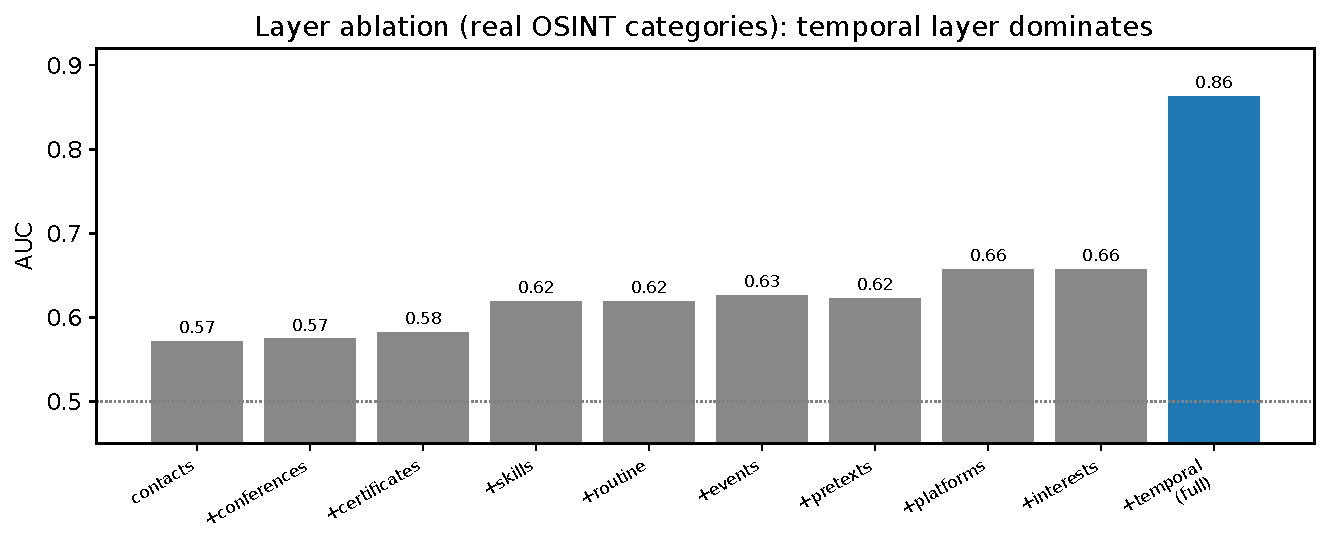
\includegraphics[width=0.9\textwidth]{fig_ablation.pdf}
\caption{Kumulatywna ablacja warstw (\texttt{exp\_ablation.csv}):
osiem warstw OSINT dokłada mało ponad kontakty ($0{,}57\to0{,}66$),
cecha spójności czasowej niesie resztę sygnału ($\to0{,}86$).}
\label{fig:m-ablation}
\end{figure}

\begin{figure}[htbp]\centering
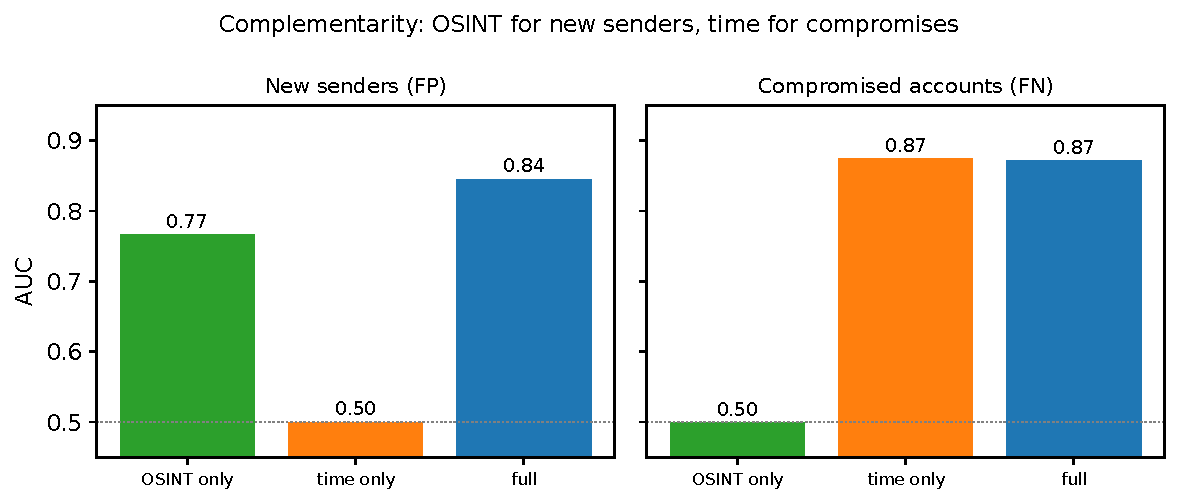
\includegraphics[width=0.9\textwidth]{fig_layer_by_threat.pdf}
\caption{Ablacja grupowa per zagrożenie: dla nowych nadawców
krytyczny jest OSINT, czas bezużyteczny; dla przejęć --- odwrotnie
(\texttt{exp\_layer\_by\_threat.csv}).}
\label{fig:m-bythreat}
\end{figure}

\section{Wyniki: uczciwa kontrola OSINT i tc-split}
\label{sec:m-osint}

Kontrola tasująca \emph{wszystkie} cechy nie izoluje wkładu samych
warstw OSINT; dlatego stosujemy kontrolę tasującą \emph{tylko}
warstwy OSINT (kontakty i rytm nietknięte) oraz nowy podział
\emph{tc-split}, który lokalizuje margines OSINT na plasterkach
konsystencji czasowej. Wyniki (\texttt{exp\_osint\_shuffle.csv},
\texttt{exp\_tc\_split.csv}):

\begin{itemize}
\item pełny multipleks $0{,}857$ [CI $0{,}852$--$0{,}863$]; bez OSINT
(kontakty+rytm) $0{,}826$; z tasowanym OSINT $0{,}821$; z tasowanym
wszystkim $0{,}503$. Wniosek: zysk niosą kontakty i rytm, a OSINT
dokłada $\sim\!0{,}03$ AUC --- i tasowanie tylko OSINT ten margines
zabiera;
\item na plasterku \emph{znany nadawca} multipleks nic nie zmienia
($0{,}79\approx0{,}79$); na plasterku \emph{w rytmie} (atak
w mimikrii) $0{,}58\to0{,}64$; na plasterku \emph{nowy nadawca}
$0{,}81\to0{,}90$ (czułość@1\% $0{,}11$) --- a tasowanie OSINT
cofa oba plasterki, więc jest to przyczynowy wkład OSINT;
\item wartość metody leży jednak po stronie fałszywych alarmów:
detekcja zimnej impersonacji pozostaje słaba (czułość $0{,}04$
przy FPR~1\%); OSINT służy do \emph{unieważniania} legalnych
nowych nadawców, nie do wykrywania podszywek.
\end{itemize}

\section{Wyniki: dekorelacja topologii}
\label{sec:m-topologia}

Prawie-tożsamość warstw strukturalnych
(kontakty$\approx$hierarchia$\approx$domena, Jaccard $\ge0{,}9$)
jest artefaktem generatora, który przypisuje jedną domenę na firmę.
Pokrętło dekorelacji $\rho$ przestraja kontakty między firmami
(\texttt{exp\_topology\_correlation.csv}): przy $\rho=0{,}8$
Jaccard spada do $0{,}39$, a niezależny wkład warstw strukturalnych
rośnie z $0{,}02$ do $0{,}25$ AUC --- znalezisko „efektywnie 3--4
niezależne warstwy" jest więc własnością zwartej populacji, nie
metody multipleks.

\section{Wyniki: realistyczna fabrykacja śladów}
\label{sec:m-fabrykacja}

Atakujący może sfabrykować ślad OSINT. Stwierdzenie~\ref{prop:fab}
przewiduje: przy fabrykacji i.i.d.\ z rozkładu \emph{prawdziwych}
śladów cechy istnienia tracą moc, kontrola permutacji ofiar jest
odporna na tempo fabrykacji, a zostają tylko cechy \emph{spójności}.
Pomiar (\texttt{exp\_multiplex.csv}, sweep fabrykacji;
tab.~\ref{tab:m-fab}): AUC multipleksu eroduje stopniowo
$0{,}88\to0{,}84$ ($10\%$ fałszywych krawędzi) $\to0{,}79$
($25\%$) $\to0{,}70$ przy $50\%$ --- poziomu samych kontaktów ---
z częściowym odbiciem $0{,}81$ przy $100\%$, gdy każdy atak niesie
ślad wyglądający na prawdziwy i rozdzielają już tylko rezydualne
sprzężenia; fałszywe alarmy na nowych nadawcach wracają od
$25\%$ fabrykacji. Kontrola tasowania pozostaje płaska
$0{,}50\pm0{,}01$ w całym zakresie --- zgodnie z częścią (ii)
stwierdzenia. Dla kontrastu, fabrykator \emph{legacy} (dowolna
warstwa, honorowana per zdarzenie) podnosi kontrolę tasowania
z tempem fabrykacji ($0{,}50\to0{,}60$ przy $50\%$;
\texttt{exp\_sweep\_fab.csv}) --- artefakt naruszenia (ii).

\begin{table}[htbp]\centering
\begin{tabular}{lcccccc}
\toprule
Fabrykacja OSINT & $0\%$ & $10\%$ & $25\%$ & $50\%$ & $75\%$ & $100\%$ \\
\midrule
AUC multipleksu   & $0{,}88$ & $0{,}84$ & $0{,}79$ & $0{,}70$ & $0{,}73$ & $0{,}81$ \\
Kontrola tasowania & $0{,}51$ & $0{,}50$ & $0{,}50$ & $0{,}50$ & $0{,}50$ & $0{,}50$ \\
\bottomrule
\end{tabular}
\caption{Realistyczna fabrykacja śladów (20 ziaren;
\texttt{exp\_multiplex.csv}): marża eroduje stopniowo do poziomu
samych kontaktów przy $50\%$ z częściowym odbiciem przy $100\%$,
zgodnie ze stw.~\ref{prop:fab}(i)+(iii); kontrola tasowania płaska
--- część (ii).}
\label{tab:m-fab}
\end{table}

\section{Wyniki: realny Enron i pułapka wycieku rytmu}
\label{sec:m-enron}

Z nagłówków korpusu Enron \citep{klimt2004enron} budujemy
\emph{realny} multipleks strukturalno-czasowy na $818$ nadawcach
i $\sim\!170$k zdarzeń: kontakty, współodbiorcy (konta adresowane
razem), ta sama domena pocztowa oraz rytm nadawcy --- wszystko
z samych nagłówków, \emph{bez} warstw OSINT (świadomy podział,
który trzyma wynik realny wolnym od syntetycznych nakładek).
Rytm estymujemy na dwa sposoby: z \emph{pełnej} historii --- co
wycieka okres ewaluacji do estymatu (cecha nieprzyczynowa,
def.~\ref{def:causal-feature}) --- albo z \emph{wczesnych} $60\%$
okresu z ewaluacją na późniejszych $40\%$ (uczciwy podział
czasowy); audyt off-hours wprawia frakcję legalnej poczty poza
estymowanym rytmem.

Tabela~\ref{tab:m-enronsplit} jest wynikiem metodologicznym
rozdziału. Pod wyciekającą estymacją samej warstwy czasowej,
detektor rytmu raportuje pozorną czułość $0{,}73$@FPR$1\%$;
pod uczciwym podziałem czasowym --- \emph{$0{,}00$ nawet przy
FPR~$5\%$}, bo ponad $5\%$ legalnej poczty wypada poza uczciwie
policzonym rytmem (próg nie spełnia FPR$\le1\%$ i czułość
jednobitowej cechy spada skokowo do zera, choć AUC jest wciąż
$0{,}75$). Pełny multipleks zachowuje czułość $0{,}14$
(AUC $0{,}82$), a z ruchem off-hours --- $0{,}01$--$0{,}15$
(AUC $0{,}77$): warstwy strukturalne liczone z wczesnych $60\%$,
jak rytm. Zgodnie z twierdzeniem~\ref{thm:lookahead} luka
$(0{,}73\to0{,}00)$ jest dokładnie obciążeniem look-ahead:
estymacja rytmu nadawcy na okresie ewaluacji daje pozorną
czułość, która znika pod kontrolą przyczynowości. To ostrzeżenie
dla całej klasy detektorów behawioralnych: \emph{każdy} rytm,
profil aktywności czy baseline liczony na pełnej historii zawyża
czujność detektora, który potem jest na nim ewaluowany.

\begin{table}[htbp]\centering
\begin{tabular}{lcccc}
\toprule
& \multicolumn{2}{c}{warstwa czasowa} & \multicolumn{2}{c}{pełny multipleks} \\
\cmidrule(lr){2-3}\cmidrule(lr){4-5}
Rytm estymowany z & AUC & cz.@1\% & AUC & cz.@1\% \\
\midrule
pełnej historii (\emph{z wyciekiem})   & $0{,}86$ & $0{,}73$ & $0{,}94$ & $0{,}88$ \\
wczesnego okna (\emph{podział czasowy}) & $0{,}75$ & $0{,}00$ & $0{,}82$ & $0{,}14$ \\
wczesnego okna $+$ off-hours (\emph{oba}) & $0{,}68$ & $0{,}00$ & $0{,}77$ & $0{,}01$ \\
\bottomrule
\end{tabular}
\caption{Kontrola wycieku rytmu na realnym grafie Enron (20 ziaren;
\texttt{exp\_enron\_temporal\_split.csv}): estymacja rytmu na pełnej
historii zawyża warstwę czasową do pozornej czułości $0{,}73$;
uczciwy podział czasowy sprowadza ją do $0{,}00$, podczas gdy pełny
multipleks trzyma $0{,}14$ (bez off-hours).}
\label{tab:m-enronsplit}
\end{table}

\begin{figure}[htbp]\centering
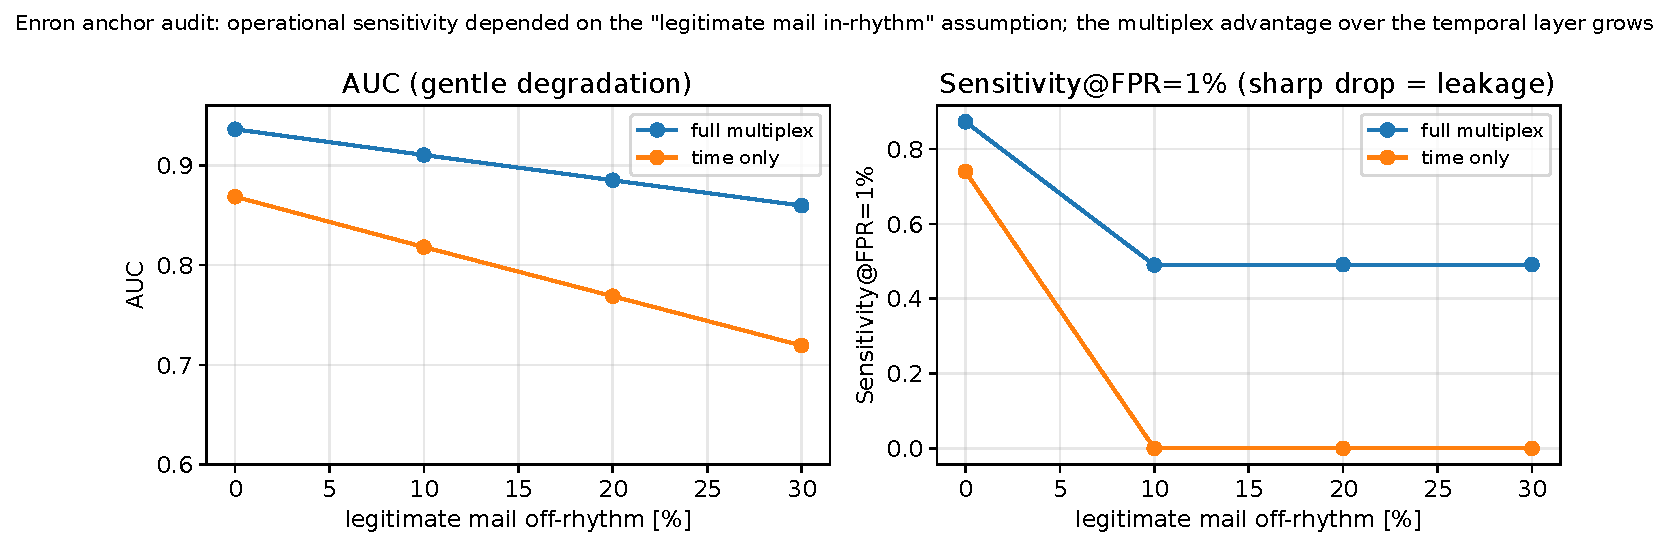
\includegraphics[width=0.9\textwidth]{fig_enron_audit.pdf}
\caption{Audyt Enron: AUC degraduje łagodnie z frakcją ruchu
poza godzinami pracy, ale operacyjna czułość@FPR$1\%$ warstwy
czasowej bez podziału czasowego była zawyżona --- po usunięciu
wycieku spada do zera, a przewaga multipleksu rośnie z frakcją
off-hours (paczka reprodukcyjna).}
\label{fig:m-enronaudit}
\end{figure}

\section{Wyniki: narażenie detektorowo-relatywne}
\label{sec:m-susc}

Tabela~\ref{tab:m-susc} rozkłada chybienia detektora fuzji
(czułość@FPR$1\%$, 20 ziaren, bootstrapowe 95\% CI) per kanał
ataku i starszeństwo ofiar. \emph{Kanał, nie ranga, napędza
narażenie}: zimna impersonacja zewnętrzna zostawia strukturalną
podłogę $\mathrm{Susc}\approx0{,}96$ na \emph{każdym} poziomie ---
bo żadna warstwa nie pokrywa nadawcy spoza grafu; przejęte konto
jest mniej groźne ($0{,}855$), bo znany kontakt poza rytmem to
ostre, nisko-FP sprzężenie. W kanale lateral obserwujemy ---
ale nie ogłaszamy jako odkrycia --- porządek odwrotny wobec
intuicji, że bogatsze osadzenie w grafie chroni: executive,
najbogatsi w warstwach wiedzy domenowej, są \emph{najbardziej}
narażeni ($\mathrm{Susc}=0{,}924$), juniorzy i mid-level
najmniej ($0{,}840$/$0{,}838$). Plauzybilne wyjaśnienie: bogato
osadzona ofiara ma dużo legalnej poczty poza rytmem i dużo
kontaktów międzywarstwowych, co poszerza przestrzeń, w której
atak wygląda na spójny. Powód ostrożności jest konstrukcyjny:
generator wiąże bogactwo warstw ze starszeństwem, więc kierunek
porządku części wynika z tego sprzężenia i wymaga testu pod
alternatywnymi przypisami. Tym, co twarde, jest: kanał dominuje
rangę, a starszeństwo nie kupuje ochrony.

\begin{table}[htbp]\centering\small
\begin{tabular}{llcc}
\toprule
Wymiar & Grupa & cz.@1\% & $\mathrm{Susc}$ \\
\midrule
\multirow{2}{*}{Kanał}
 & Impersonacja zewn. (zimne BEC) & $0{,}038$ & $\mathbf{0{,}962}$ \\
 & Przejęte konto (lateral)       & $0{,}145$ & $0{,}855$ \\
\midrule
\multirow{4}{*}{Starszeństwo (lateral)}
 & Executive & $\mathbf{0{,}076}$ & $\mathbf{0{,}924}$ \\
 & Senior    & $0{,}135$ & $0{,}865$ \\
 & Mid-level & $0{,}162$ & $0{,}838$ \\
 & Junior    & $0{,}160$ & $0{,}840$ \\
\midrule
\multirow{4}{*}{Starszeństwo (zimne BEC)}
 & Executive & $0{,}038$ & $0{,}962$ \\
 & Senior    & $0{,}040$ & $0{,}960$ \\
 & Mid-level & $0{,}042$ & $0{,}958$ \\
 & Junior    & $0{,}035$ & $0{,}965$ \\
\bottomrule
\end{tabular}
\caption{Narażenie detektorowo-relatywne detektora fuzji
(\texttt{exp\_susceptibility.csv}; 20 ziaren, FPR $=1\%$; 95\%
bootstrap CI po ziarnach --- patrz CSV): kanał ataku, nie ranga
ofiar, napędza narażenie; zimna impersonacja zostawia podłogę
$\approx0{,}96$ na każdym stanowisku.}
\label{tab:m-susc}
\end{table}

\section{Wyniki: granica graf--treść}
\label{sec:m-tresc}

Bo niezmiennik jest ślepy na zimną impersonację spoza grafu,
przypadek ten jest domeną treści. Eksperyment fuzji
(\texttt{exp\_content\_fusion.csv}; tab.~\ref{tab:m-tresc}) w dwóch
reżimach: w reżimie \emph{tell-tale} (atak z błędem treściowym)
treść (TF-IDF) rozdziela niemal idealnie ($0{,}997$) i multipleks
jest zbędny; w reżimie \emph{mimikrii} (BEC) treść jest ślepa
($0{,}496$), a sygnał niesie multipleks ($0{,}859$). Fuzja trzyma
się blisko lepszej modalności w każdym reżimie ($0{,}998$,
odpowiednio $0{,}851$) --- potwierdza, że treść i graf zawodzą
na \emph{różnych} atakach i że ich fuzja kosztuje mało; argument
za systemem hybrydowym. Jako sanity-check: na tym małym grafie
pojedynczy niestrojony multiplex GNN nie przewyższa jawnych cech
ręcznych (AUC $0{,}78$ wobec $0{,}86$ dla gradient boostingu) ---
w tej skali jawnie zdefiniowane cechy przynależności już łapią
sygnał.

\begin{table}[htbp]\centering
\begin{tabular}{lccc}
\toprule
Reżim & Treść & Multipleks & Fuzja \\
\midrule
Tell-tale (ślad w treści) & $0{,}997$ & $0{,}859$ & $\mathbf{0{,}998}$ \\
Mimikria (BEC)            & $0{,}496$ & $\mathbf{0{,}859}$ & $0{,}851$ \\
\bottomrule
\end{tabular}
\caption{Fuzja treści (TF-IDF) z multiplexem (AUC, 20 ziaren;
\texttt{exp\_content\_fusion.csv}): treść i graf zawodzą na
różnych atakach; fuzja trzyma się blisko lepszego w każdym
reżimie.}
\label{tab:m-tresc}
\end{table}

\section{Graf wiedzy domenowej jako narzędzie i cel}
\label{sec:m-kg}

Formalizm z sekcji~\ref{sec:m-model} nie jest li tylko aparatem
detekcji --- jego obiekt, graf wiedzy, jest coraz popularniejszym
\emph{narzędziem} do zapisywania wiedzy, w tym notatek. Ta sekcja
krótko sytuuje rozdział w tym kontekście i pokazuje, że jego
wyniki czytają się tam jako: mapa dla atakującego, cel ataku
i zasada detekcji anomalii.

\paragraph{Grafy wiedzy jako narzędzie.} Grafy wiedzy są
dojrzałym paradygmatem reprezentacji wiedzy \citep{hogan2021knowledge,
ji2022survey}: od otwartych grafów encyklopedycznych po
organizacyjne grafy wiedzy i tematyczne --- w tym grafy wiedzy
o zagrożeniach (CTI) budowane wspomaganie modelami językowymi
\citep{fieblinger2024actionable,cheng2024ctinexus}. W warstwie
osobistej i zespołowej grafowa struktura notatek stała się
standardem narzędzi typu \emph{second brain} (Obsidian, Logseq,
Roam): notatka jest węzłem, a konspektyczny link --- krawędzią;
w efekcie graf NOTATEK organizacji jest często cichym, bogatym
\emph{shadow} tego samego grafu wiedzy domenowej, który
aksjomatyzujemy w definicji~\ref{def:m-dkg}. Trzeci nurt ---
fuzja z modelami językowymi: grafy wiedzy osadzone w
architekturach GraphRAG i pamięci agentów jako warstwa
wierzygodnego kontekstu \citep{pan2024roadmap,edge2024graphrag}
--- czyni z grafu wiedzy nie tylko nośnik notatek, ale czynnik
\emph{decyzyjny}: odpowiedź systemu jest tak dobra, jak
wierzygodność krawędzi, z których ją zretrievowano.

\paragraph{Ta sama struktura jest mapą dla atakującego.}
Wszystko, co w grafie wiedzy organizacji jest pomocne --- kim
jest dany pracownik, z kim pracuje, o czym pisze, w jakim rytmie
--- jest też dokładnie materiałem OSINT, z którego atakujący
buduje pretekst (sekcja~\ref{sec:p-osint}; \citealp{edwards2017panning,
brown2025web}). Graf publikowany, udostępniany na zewnątrz
albo rekonstruowalny ze śladów (konferencje, certyfikaty,
profile) jest \emph{mapą ataku}: personalizacja, która kiedyś
wymagała wiedzy eksperckiej, sprowadza się do zapytań po
grafie. Model zagrożeń tego rozdziału bierze to explicite:
atakujący zna warstwy i może w nie celować.

\paragraph{Jest też celem ataku.} Gdy graf wiedzy zasila detekcję
lub GraphRAG, kontrola nad krawędziami jest kontrolą nad
decyzją. Wektorami są: (i)~\emph{fabrykacja krawędzi} --- dodanie
do publicznego śladu faktów łączących atakującego z ofiarą,
podnoszenie spójności międzywarstwowej; twierdzenie
\ref{prop:fab} i sweep z sekcji~\ref{sec:m-fabrykacja} pokazują
właśnie ten mechanizm: do $\sim\!50\%$ fałszywych krawędzi
marża detektora eroduje do poziomu samych kontaktów, a przy
pełnej fabrykacji każdy atak niesie ślad nierozróżnialny
od prawdziwego; (ii)~\emph{trucie korpusu i osadzeń} ---
literatura ataków adversarialnych na grafy pokazuje, że
dodanie kilku starannie dobranych krawędzi zmienia klasyfikację
GNN \citep{zugner2018adversarial,zugner2019adversarial,
dai2022towards}; jeśli obrona działa na grafie, który atakujący
może wzbogacić, nieprzyczynowe cechy (def.~\ref{def:causal-feature})
i kontrola tasowania (stw.~\ref{prop:shuffle}) są warunkiem
oznaczenia ataku, nie opcją; (iii)~\emph{iniekcja treści} ---
w architekturach RAG dokument wciągnięty do korpusu staje się
przyszłą „wiedzą", którą system przywoła jako kontekst;
zatruty dokument to odpowiednik sfałszowanej notatki
w grafie wiedzy.

\paragraph{Zasada detekcji anomalii uogólnia się.} Niezmiennik
rozdziału --- prawdziwa relacja jest spójna w wielu warstwach
naraz --- jest w istocie ogólną zasadą detekcji anomalii
na grafach wiedzy i notatkach: encja, notatka lub krawędź,
która pojawia się w jednej warstwie i jest przeczona przez
pozostałe (kontakty, hierarchia, rytm, treść notatek), jest
sygnałem anomalii --- tak detekują oszustwa metody
niespójności między perspektywami \citep{liu2020alleviating},
a szersza rodzina nienadzorowanych detektorów anomalii
grafowych \citep{akoglu2015graph,liu2021anomaly,li2025umgad,
behrouz2022anomaly} czyta ten sam wzorzec. Praktyczna reguła
dla narzędzi notatek i CTI-graphów brzmi więc tak, jak brzmi
protokół rozprawy: (a)~warstwa za warstwą, z jawną wagą ufności
$w_L$ i rytem $\tau$; (b)~ocena spójności wielowarstwowej zamiast
pojedynczych flag; (c)~każda cecha i każdy baseline liczony
wyłącznie z przeszłości (tw.~\ref{thm:lookahead}); (d)~kontrola
fabrykacji sprawdzająca, ile fałszywych krawędzi eroduje marżę
(stw.~\ref{prop:fab}). Z oddali: wandalizm --- celowe wstawianie
fałszywych tez --- jest operacyjną rzeczywistością publicznych
grafów wiedzy, z własnym torem detekcji
\citep{heindorf2017wsdmcup,sarabadani2017tools,heindorf2019debiasing}
i korpusami historii rewizji \citep{schmelzeisen2022wikidated};
trucie grafów GraphRAG (recepta PoisonedRAG przeniesiona na
konstrukcję grafu) pokazuje, że „kilka słów zniekształca graf"
\citep{wen2025fewwords,kepo2026,zou2024poisonedrag}, a wstrzyknięcie
pośrednie pozwala odzyskanemu zatrutemu dokumentowi stać się
instrukcją dla modelu \citep{greshake2023not}.

\paragraph{Trzy pomiary artykułu C.} Ten obraz jest mierzalny w paczce
reprodukcyjnej (artykuł C; \texttt{exp\_fab\_edge\_detection.csv},
\texttt{exp\_rag\_poison.csv}, \texttt{exp\_kg\_poisoning.csv}):
(i)~przy fabrykacji i.i.d.\ z rozkładu łącznego prawdziwych śladów
detekcja \emph{krawędziowa} jest bezradna --- cechy istnienia AUC
$\approx0{,}50$, kontrola permutacji $0{,}50$, a pozorny sygnał
spójności ($0{,}56$--$0{,}65$) jest artefaktem definicji
prawdziwości, który rozprawa ujawnia jawnie (empiryczna granica
stw.~\ref{prop:fab}(i)--(iii)); (ii)~w retrieval GraphRAG-lite atak
zoptymalizowany pod zapytanie (recepta PoisonedRAG) korumpuje $100\%$
top-5 ofiar, a bramka spójności (wsparcie w warstwach wewnętrznych
LUB $\ge2$ niezależne ślady OSINT) zeruje go --- podnosząc koszt
atakującego z jednego wstrzykniętego tekstu do $\ge2$ niezależnych
sfałszowanych publicznych śladów na ofiarę, przy cenie $92{,}5\%$
oflagowanych legalnych międzyorganizacyjnych jedno-faktowych
więzi na czystym korpusie; (iii)~na publicznym FB15k-237 spójność
relacyjna ranguje sfabrykowane trójki na AUC $0{,}72$ (cechy
istnienia $0{,}52$; kontrast sparowany Wilcoxon $p{=}0{,}005$,
$\delta{=}1{,}0$), ale sens@FPR$1\%\approx0$ --- podłoga
izolowanych trójek prawdziwych czyni z niej narzędzie triażu,
nie filtr progowy, zgodnie z regułą bazy rozdziału formalnego;
a fabrykator \emph{path-preserving}, który zna cechę wspólnych
sąsiadów i kopiuje mierzoną przez nią własność, neutralizuje ją
(AUC $0{,}71\to0{,}56$) --- wyścig zbrojeń jest cecha po cecha,
przetrwać może tylko potwierdzenie przez własności, które
atakujący musi skopiować łącznie.

\section{Podsumowanie rozdziału}
\label{sec:m-podsumowanie}

\paragraph{RQ3 (sygnał międzywarstwowy).} Niespójność międzywarstwowa
jest rzeczywistym sygnałem na grafie studyjnym: fuzja warstw z rytmem
podnosi AUC $0{,}70\to0{,}88$ i likwiduje $100\%$ fałszywych alarmów
na legalnych nowych nadawcach, kontrola tasowania spada do losowego
($0{,}51$), a uczciwa kontrola tylko-OSINT i tc-split lokalizują
margines OSINT ($+0{,}03$ AUC globalnie; $0{,}81\to0{,}90$ na
plasterku nowych nadawców; zysk z tasowania OSINT znika). Uczciwe
znalezisko: cecha spójności czasowej niesie większość sygnału
rankingowego, warstwy strukturalne są na zwartej populacji prawie
współliniowe (Jaccard $0{,}93$; po dekorelacji $\to0{,}39$ ich
niezależny wkład rośnie do $0{,}25$). Wartość praktyczna metody
leży po stronie fałszywych alarmów, nie czujności na podszywki
(zimna impersonacja: $0{,}04$@1\%).

\paragraph{RQ4 (narażenie i granice).} Miara narażenia
detektorowo-relatywnego pokazuje, że narażenie napędza kanał ataku,
nie ranga ofiar (zimna impersonacja: podłoga $\approx0{,}96$ na
każdym stanowisku; w kanale lateral executive najbardziej narażeni
--- $0{,}924$ --- a bogactwo osadzenia nie kupuje ochrony);
treść i graf zawodzą na różnych atakach i ich fuzja jest blisko
lepszego z nich w każdym reżimie. Granice ewaluacji tej klasy
detektorów ujawnia pułapka wycieku rytmu: pozorna czujność
$0{,}73$@1\% detektora rytmu estymowanego na pełnej historii
spada do $0{,}00$ pod uczciwym podziałem czasowym, podczas gdy
multipleks trzyma $0{,}14$ --- empiryczna instancja
twierdzenia~\ref{thm:lookahead} i praktyczna reguła: rytm, profil
i baseline behawioralny estymować wyłącznie z okresu
\emph{poprzedzającego} ewaluację.

% =====================================================================
% ROZDZIAŁ 6 — Synteza
% =====================================================================
\chapter{Synteza: twierdzenia, pomiary i implikacje operacyjne}
\label{rozd:synteza}

\section{Od warunków do wyników: jedna tablica}
\label{sec:s-mapa}

Rozdziały empiryczne nie są ilustracjami do rozdziału formalnego ---
jego twierdzenia zostały \emph{sformułowane pod} pomiarami, a każdy
warunek ma swoją empiryczną instancję w paczce reprodukcyjnej.
Tablica~\ref{tab:mapping} (rozdz.~\ref{rozd:formalny}) zamyka
mapowanie; tu zbieramy jego wnioski po obu stronach.

\paragraph{Warunek (a): przyczynowość zdarzeniowa cech.} Usunięcie
wycieków (momentum liczone z przeszłych okien, liczniki wolumetryczne
tylko z kubełków przeszłych, cechy stopni GNN ze splitu
treningowego) poprzedziło przeliczenie wszystkich wyników --- i jest
operacyjnie testowalne (\texttt{tests/test\_causality.py}: cecha
jest przyczynowa wtedy i tylko wtedy, gdy usunięcie przyszłości nie
zmienia jej wartości). Empiryczna dywidenda: po naprawie pozorna
czułość rytmu $0{,}73$@1\% okazała się wartością $0{,}00$ pod
uczciwym podziałem (rozdz.~\ref{sec:m-enron}) --- rzędy wielkości
zawieszenia między wersją wyciekającą a uczciwą to najdokładniejszy
pomiar ceny warunku (a) w całej rozprawie.

\paragraph{Warunek (b): podział po ofiarach i organizacjach.}
Bez rozłączności ofiar cechy agregujące po otoczeniu ofiary
wykorzystują zdarzenia ataku z okresu ewaluacji w treningu
(stw.~\ref{prop:split}). Podział indukcyjny po organizacjach
(rozdz.~\ref{sec:k-stabilnosc}) pokazuje dodatkowo, że miarą
jest wtedy \emph{transfer ryzyka}: cechy wolumetryczne
transferują się najlepiej, sygnał odbiorczy degraduje --- zmiana
protokołu zmienia ranking detektorów, więc protokół jest częścią
wyniku, nie tłem.

\paragraph{Warunek (c): usunięcie sygnatury iniekcji.} Sonda KS
mierzy czysto czasowy brzeg sygnału (lemat~\ref{lem:probe}); po
zastąpieniu odstępów iniekcji rozkładem tła detektor temporalny
zachowuje marżę $+0{,}10$ AUC nad wolumetrycznym (Enron
$0{,}77$ wobec $0{,}67$), podczas gdy cechy ręczne spadają do
poziomu wolumetrycznego --- marża, która przeżywa, jest sygnałem
interakcyjnym (tw.~\ref{thm:injection}).

\paragraph{Warunek (d): realistyczna fabrykacja.} Sweep fabrykacji
rozdziału~\ref{sec:m-fabrykacja} pokazuje erozję stopniową
($0{,}88\to0{,}70$ przy $50\%$) z płaską kontrolą tasowania ---
zgodnie ze stw.~\ref{prop:fab}; kontrast z fabrykatorem legacy,
który podszywał samą kontrolę, pokazuje, że (d) jest warunkiem
\emph{wymagającym}, nie kosmetycznym.

\section{Sygnał w jednym zdaniu}
\label{sec:s-sygnal}

Po odjęciu wszystkiego, co wycieka, sygnał, który zostaje,
jest jednego rodzaju: \emph{sparcie czasu ze strukturą grafu}
--- fala po stronie odbiorców kaskady (rozdz.~\ref{rozd:kaskada})
i spójność międzywarstwowa wobec prawdziwego pokrycia nadawcy
(rozdz.~\ref{rozd:multipleks}). Sam brzeg czasowy jest
bezużyteczny (rhythm-only $0{,}50$; po zastąpieniu sygnatury
sonda spada do $0{,}54$--$0{,}63$), sama topologia jest
niewystarczająca (statyczny GNN $0{,}76$ z czułością $0{,}039$),
a sam sygnał ma mierzalne granice: fan-out $\ge2$ (punkt ślepy),
szum etykiet (nauczony model degraduje najszybciej), prewalencja
(triage, nie autonomiczna obrona).

\section{Implikacje operacyjne dla SOC}
\label{sec:s-soc}

\paragraph{Co monitorować.} Fala odbiorcza jest własnością grafu
komunikacji organizacji, policzalną z samych nagłówków --- pasuje do
wewnętrznego pipeline'u triażu nie otwierającego treści. Rytm
i profil behawioralny estymować wyłącznie z okna poprzedzającego
okres oceny; każde rozszerzenie okna estymacji na okres oceny
zawyża czujność rzędami wielkości.

\paragraph{Gdzie monitor zawodzi.} Punkt ślepy jest konkretny:
pojedyncza prośba o przelew z przejętego konta jest niewidoczna
dla każdego badanego detektora --- kontrola procesowa poza
kanałem (out-of-band) pozostaje warunkiem koniecznym, a detektor
kaskadowy ma ją \emph{uzupełniać}, nie zastępować. Zimna
impersonacja spoza każdej warstwy zostawia narażenie
$\approx0{,}96$ na każdym stanowisku --- tam musi działać treść
i proces, co potwierdza fuzja (blisko lepszego w każdym reżimie).

\paragraph{Jak czytać liczby.} Przy realnej prewalencji $1{:}10^4$
i punkcie pracy (czułość $0{,}10$; FPR $1\%$) każde wykrycie niesie
$\sim\!10^3$ fałszywych alarmów, w reżimie skrytym $\sim\!3300$;
punkt pracy jest trzy rzędy wielkości od progu produkcyjnego
($4\cdot10^{-6}$, \citealp{ho2019detecting}). Detektory tej klasy
są narzędziem rankingu dla analityków: ich wartość operacyjna
mierzy się redukcją obciążenia analityka przy stałym budżecie
alertów, nie samą czułością.

\paragraph{Narażenie jako wielkość projektowa.} Miara
$\mathrm{Susc}$ pozwala rozmawiać o narażeniu bez odwołań
do psychologii: kanał dominuje rangę, a bogactwo osadzenia
w grafie \emph{nie} kupuje ochrony (executive najbardziej
narażeni w kanale lateral). Dla planujących kontrole oznacza
to twardą hierarchię: najpierw kanał ataku, potem rola.

% =====================================================================
% ROZDZIAŁ 7 — Zakończenie
% =====================================================================
\chapter{Zakończenie}
\label{rozd:zakonczenie}

\section{Odpowiedzi na pytania badawcze}
\label{sec:z-rq}

\paragraph{RQ1 (sygnał kaskadowy).} Tak: przejęte konto zgodne
z każdą statyczną relacją jest wykrywalne z dynamiki kaskady.
Hierarchia detektorów jest jednoznaczna (1-hop $0{,}70$; GNN
statyczny $0{,}76$; ręczny kontekst $0{,}81$; temporalny GNN
$0{,}87$ z czułością operacyjną $0{,}099$@1\%), przewaga jest
temporalna w sensie ablacyjnym (tasowanie: $0{,}87\to0{,}73$)
i przenosi się kierunkowo na trzy realne grafy (Enron: temporalny
$0{,}85$, czułość $0{,}215$ pod atakiem skrytym, przy czułości
$0{,}000$ detektora wolumetrycznego; SNAP: kontrast reżimowy
replikowany w kierunku na obu grafach).

\paragraph{RQ2 (granice).} Sygnał wymaga fan-outu $\ge2$ (atak
na jednego odbiorcę: AUC $\approx0{,}5$ dla każdego detektora);
propagacja nie jest konieczna (przy $p_{\mathrm{inf}}=0$ i fan-oucie
$\ge2$ wykrywalność wraca). Sygnał degraduje łagodnie ze skalą,
kurczy się pod szumem etykiet (nauczony model najszybciej:
$0{,}72\to0{,}59$ przy $20\%$), a między organizacjami najlepiej
transferują się cechy wolumetryczne. Przy realnej prewalencji
detektory są instrumentem triażu: $\sim\!10^3$ fałszywych alarmów
na wykrycie.

\paragraph{RQ3 (sygnał międzywarstwowy).} Tak: niespójność
międzywarstwowa oddziela impersonację zewnętrzną od legalnych
nowych nadawców (AUC $0{,}70\to0{,}88$, fałszywe alarmy
$100\%\to0\%$), kontrola tasowania spada do losowego, a kontrola
tylko-OSINT i tc-split lokalizują przyczynowy margines warstw
($+0{,}03$ AUC; $0{,}81\to0{,}90$ na plasterku nowych nadawców).
Uczciwa ablacja pokazuje, że większość sygnału rankingowego niesie
spójność czasowa, a wartość OSINT leży po stronie fałszywych
alarmów; sygnał eroduje pod realistyczną fabrykacją zgodnie ze
stwierdzeniem~\ref{prop:fab}.

\paragraph{RQ4 (narażenie i granice).} Narażenie napędza kanał
ataku, nie ranga ofiar: zimna impersonacja zostawia strukturalną
podłogę $\mathrm{Susc}\approx0{,}96$ na każdym stanowisku, a w kanale
lateral executive są \emph{najbardziej} narażeni --- bogactwo
osadzenia nie kupuje ochrony. Treść i graf zawodzą na różnych
atakach, a ich fuzja trzyma się blisko lepszego w każdym reżimie.
Najważniejsze odkrycie metodyczne rozprawy --- pułapka wycieku
rytmu --- pokazuje, że rytm estymowany na pełnej historii zawyża
czujność behawioralną z $0{,}00$ (uczciwie) do $0{,}73$ (z
wyciekiem): miara ceny naruszenia warunku przyczynowości
na realnym korpusie.

\section{Wkład rozprawy}
\label{sec:z-wklad}

Rozprawa wnosi: (i)~ramę formalną ewaluacji strumieniowej ---
klasę cech i detektorów zdarzeniowo-przyczynowych, cztery
mechanizmy wycieku jako twierdzenia z konstrukcyjnymi
kontrprzykładami, dekompozycję wyniku detektora na składową
czysto czasową i sprzęgającą czas z grafem, wynik o
nierozróżnialności śladów przy realistycznej fabrykacji
(rozdz.~\ref{rozd:formalny}); (ii)~pomiar i formalizację lateral
phishingu jako naruszenia grafu komunikacji w czasie --- z
odbiorczą falą kaskady jako niezmiennikiem, atakującym skrytym
jako testem krytycznym i replikacją na trzech realnych
topologiach (rozdz.~\ref{rozd:kaskada}); (iii)~pomiar
i formalizację impersonacji zewnętrznej jako naruszenia grafu
wiedzy domenowej --- multipleks, niespójność międzywarstwowa,
narażenie detektorowo-relatywne i granica graf--treść
(rozdz.~\ref{rozd:multipleks}); (iv)~metodologię ewaluacji
leak-aware, scalającą protokoły literaturowe z warunkami
twierdzonymi i operacjonalizowaną w paczce reprodukcyjnej, z
jawną arytmetyką bazy i granicami wypowiedzianymi
(rozdz.~\ref{rozd:synteza}).

\section{Ograniczenia}
\label{sec:z-ograniczenia}

Złośliwość jest syntetyczna: żaden publiczny korpus nie łączy
realnych kont z etykietowanymi przejęciami i ich propagacją, więc
walidujemy mechanizm (rozłożona w czasie kaskada separuje się
od ruchu legalnego dynamiką odbiorczą), nie detekcję realnych
intruzów; warstwy OSINT są syntetyczne także na realnym grafie.
Parametry kaskady i pacing są nasze; swepy pokazują stabilność
hierarchii, ale atak single-recipient pozostaje poza sygnałem
z konstrukcji. Skala jest ograniczona ($N{=}150$ w studium;
realne grafy do $\sim\!2$k węzłów), a graf studyjny jest gęstszy
niż typowa poczta korporacyjna --- nośnikiem mechanizmu poza
tym ustawieniem są replikacje Enron/SNAP, z zastrzeżeniem
kierunkowym (3--8 ziaren). Próg operacyjny pozostaje otwarty:
nawet najlepszy punkt pracy jest rzędy wielkości od progu
produkcyjnego ($<\!4$ FP/M); raportujemy tę lukę jako wymaganie
otwarte, nie rozwiązane.

\section{Kierunki przyszłej pracy}
\label{sec:z-przyszla}

Najbliższy krok to walidacja na korpusie z etykietowanymi,
\emph{realnymi} przejęciami --- zamiana dowodu mechanizmu
w pomiar wykrywalności. Model zagrożeń wymaga presji
adaptacyjnej: atakujący, który \emph{uczy się} grafu komunikacji
i dostosowuje pacing oraz wzorzec propagacji, by zejść pod falę
odbiorczą, wraz z dryfem populacji \citep{pendlebury2019tesseract}.
Po stronie modelowania: bogatszy kontekst relacyjny --- hierarchia,
kompetencje i publiczny ślad jako warstwy na tych samych kontach ---
i synteza obu kanałów w jednym detektorze fuzji graf--treść.
Po stronie ewaluacji: rozdział formalny sugeruje naturalne
rozszerzenia --- kontrola tasowania per kubełek (izolująca
czystą składową porządku od ko-występowania) oraz fabrykator
optymalizujący spójność, nie istnienie śladów. Wynik odbiorczy
jest naturalnym wejściem do kolejki triażu SOC --- pod warunkiem
ewaluacji, która wiąże go z realną redukcją obciążenia analityka
przy stałym budżecie alertów.


\bibliographystyle{unsrtnat}
\bibliography{bibliography}

\end{document}
